%%%%%%%%%%%%%%%%%%%%%%%%%%%%%%%%%%%%%%%%%%%%%%%
%%%     Declarations (skip to Begin Document, line 112, for parts you fill in)
%%%%%%%%%%%%%%%%%%%%%%%%%%%%%%%%%%%%%%%%%%%%%%%

\documentclass[10pt]{article}

\usepackage{geometry}  % Lots of layout options.  See http://en.wikibooks.org/wiki/LaTeX/Page_Layout
\geometry{letterpaper}  % ... or a4paper or a5paper or ... 
\usepackage{fullpage}  % somewhat standardized smaller margins (around an inch)
\usepackage{setspace}  % control line spacing in latex documents
\usepackage[parfill]{parskip}  % Activate to begin paragraphs with an empty line rather than an indent
\usepackage{hyperref}


\usepackage{amsmath,amssymb}  % latex math
\usepackage{empheq} % http://www.ctan.org/pkg/empheq
\usepackage{bm,upgreek}  % allows you to write bold greek letters (upper & lower case)

% for typsetting algorithm pseudocode see http://en.wikibooks.org/wiki/LaTeX/Algorithms_and_Pseudocode
\usepackage{algorithm}  

\usepackage{graphicx}  % inclusion of graphics; see: http://en.wikibooks.org/wiki/LaTeX/Importing_Graphics
% allow easy inclusion of .tif, .png graphics
\DeclareGraphicsRule{.tif}{png}{.png}{`convert #1 `dirname #1`/`basename #1 .tif`.png}
\usepackage{caption}
\usepackage{subcaption}

\usepackage{xspace}
\newcommand{\latex}{\LaTeX\xspace}

\usepackage{color}  % http://en.wikibooks.org/wiki/LaTeX/Colors

\long\def\ans#1{{\color{blue}{\em #1}}}
\long\def\ansnem#1{{\color{blue}#1}}
\long\def\boldred#1{{\color{red}{\bf #1}}}

% Useful package for syntax highlighting of specific code (such as python) -- see below
\usepackage{listings}  % http://en.wikibooks.org/wiki/LaTeX/Packages/Listings
\usepackage{textcomp}

%%% The following lines set up using the listings package
\renewcommand{\lstlistlistingname}{Code Listings}
\renewcommand{\lstlistingname}{Code Listing}

%%% Specific for python listings
\definecolor{codegreen}{rgb}{0,0.6,0}
\definecolor{codegray}{rgb}{0.5,0.5,0.5}
\definecolor{codepurple}{rgb}{0.58,0,0.82}
\definecolor{backcolour}{rgb}{0.95,0.95,0.92}
 
\lstdefinestyle{mystyle}{
    backgroundcolor=\color{backcolour},   
    commentstyle=\color{codegreen},
    keywordstyle=\color{magenta},
    numberstyle=\tiny\color{codegray},
    stringstyle=\color{codepurple},
    basicstyle=\footnotesize,
    breakatwhitespace=false,         
    breaklines=true,                 
    captionpos=b,                    
    keepspaces=true,                 
    numbers=left,                    
    numbersep=5pt,                  
    showspaces=false,                
    showstringspaces=false,
    showtabs=false,                  
    tabsize=2
}
 
\lstset{style=mystyle}
%%% End python code listing definitions

%%% Specific for matlab listings
\definecolor{dkgreen}{rgb}{0,0.6,0}
\definecolor{gray}{rgb}{0.5,0.5,0.5}
\definecolor{mauve}{rgb}{0.58,0,0.82}
 
\lstnewenvironment{matlab}[1][]{
\lstset{ %
  language=Matlab,                % the language of the code
  basicstyle=\footnotesize,           % the size of the fonts that are used for the code
  numbers=left,                   % where to put the line-numbers
  numberstyle=\tiny\color{gray},  % the style that is used for the line-numbers
  stepnumber=2,                   % the step between two line-numbers. If it's 1, each line 
                                  % will be numbered
  numbersep=5pt,                  % how far the line-numbers are from the code
  backgroundcolor=\color{white},      % choose the background color. You must add \usepackage{color}
  showspaces=false,               % show spaces adding particular underscores
  showstringspaces=false,         % underline spaces within strings
  showtabs=false,                 % show tabs within strings adding particular underscores
  frame=single,                   % adds a frame around the code
  rulecolor=\color{black},        % if not set, the frame-color may be changed on line-breaks within not-black text (e.g. commens (green here))
  tabsize=2,                      % sets default tabsize to 2 spaces
  captionpos=t,                   % sets the caption-position to top
  breaklines=true,                % sets automatic line breaking
  breakatwhitespace=false,        % sets if automatic breaks should only happen at whitespace
  title=\lstname,                   % show the filename of files included with \lstinputlisting;
                                  % also try caption instead of title
  keywordstyle=\color{blue},          % keyword style
  commentstyle=\color{dkgreen},       % comment style
  stringstyle=\color{mauve},         % string literal style
  escapeinside={\%*}{*)},            % if you want to add LaTeX within your code
  morekeywords={*,...}               % if you want to add more keywords to the set
  framexleftmargin=1mm, framextopmargin=1mm, frame=single,#1 % display caption
} }{}
%%% End matlab code listing definitions

%%%%%%%%%%%%%%%%%%%%%%%%%%%%%%%%%%%%%%%%%%%%%%%
%%%     Heading
%%%%%%%%%%%%%%%%%%%%%%%%%%%%%%%%%%%%%%%%%%%%%%%

\begin{document}

\begin{center}
    {\Large {\bf CS 665 -- Final Project Report}} \\
    Zhe Wang
    
\end{center}

%%%%%%%%%%%%%%%%
%%%     Body
%%%%%%%%%%%%%%%%
\section{Introduction}

The purpose of this project is to evaluate the Stochastic Multiresolution Persistent Homology Kernel (SMURPH) \cite{zhu2016stochastic}
This kernel tries to capture the persistence homology information of point cloud data.

In order to evaluation SMURPH kernel, I used it to calculate kernel PCA.
If the kernel is capables of what the paper claims, we should see from the 2D kernel PCA that
point clouds with similar persistence homology should form a cluster.

I conducted experiments on three different datasets. 
The first dataset is the Kitchen Utensil Dataset, which is the dataset used in the original paper.
The main reasion to use this dataset is to validate my implementation. 
If my implementation is correct, then the kernel PCA result should be at least similar to the result presented in the paper.
The other two datasets are synthetic datasets with different features. One has different number of holes and the other has different scale of holes.
Using synthetic datasets makes it easier to analyze and explain the results.

For each dataset, I also compared the kernel with two other kernels.
The first is a simple linear kernel.
This kernel serves as a base line.
Since a linear kernel shouldn't make any sense considering persistence homology of a point cloud,
we should expect the kernel PCA result don't form any clusters.
When comparing with it, we should be able to see if a kernel is capturing the persistence homology features.
The second kernel is proposed by my self, trying to come up with a simple but meaning kernel.
Basically this kernel calculate a histogram of distances (HOD) between each pair of points.
Then this histogram is used as a feature vector to calculate the inner product.

Detailed descriptions about these kernel will be presented in the following section. 


\section{Tested Kernels}

\subsection{SMURPH Kernel}
The detailed algorithm for calculating SMURPH kernel can be found in Algorithm 1 in \cite{zhu2016stochastic}.
Here I just summerize the main idea of it.
Given a point cloud, SMURPH kernel generate multiple samples at different scale: $[s_0,s_1,s_2, ..., s_n]$.
Then for each $s_i$, SMURPH build a Vietoris-Rips filtration on it and calculate the persistence diagram.
Next, the persistence diagram is converted to persistence landscape (PL) function, which becomes the representation $r_i$ for the sample $s_i$.
At last, each point cloud is represented by an array of PL functions: $[r_0, r_1, r_2..., r_n]$.
The inner product of two different point clouds becomes the inner product of two array of PL functions, which could be calculated by taking integrals.

\subsection{Linear Kernel}

A simple linear kernel is used as baseline for comparison. 
The linear kernel generate same-sized samples from given point clouds.
Then the inner product is defined as the sum of inner products of points from each sample.

\subsection{Histogram of Distances Kernel}

In order to have a meaningful yet still simple kernel for comparison,
I proposed a new kernel: Histogram of Distances (HOD).
The kernel generate a histogram of distances between each pair of points in a point cloud.
Then a histogram of the distances is calculated.
I use the normalized histogram as the vector representation of the point cloud.
So the inner product of two point clouds becomes the inner product of two vectors.
The intuition of this kernel is that point clouds don't have any holes tend to have a smooth and dense histogram of distances, while point clouds have many holes don't.


\section{Datasets}

\subsection{Kitchen Utensil Dataset}

This dataset \cite{Neumann13mlg} consists of 41 point clouds, generated by 3D scanning of kitchen utensils.
Figure ~\ref{fig:kitchen_dataset} shows two samples of this dataset.

\begin{figure}[H]
    \centering
    \begin{subfigure}[h]{0.4\textwidth}
        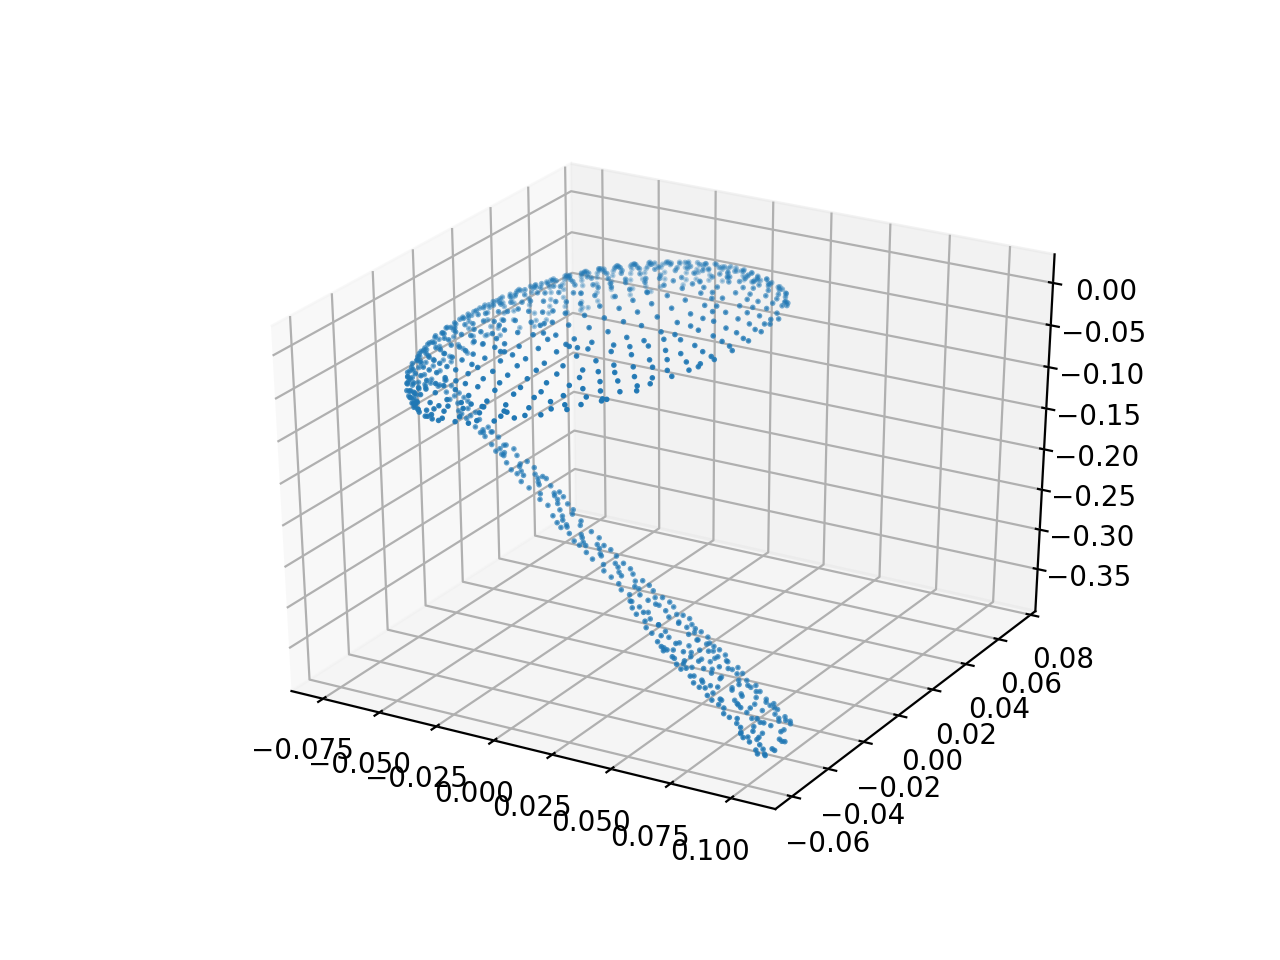
\includegraphics[width=\linewidth]{db_sample1}
    \end{subfigure}
    \begin{subfigure}[h]{0.4\textwidth}
        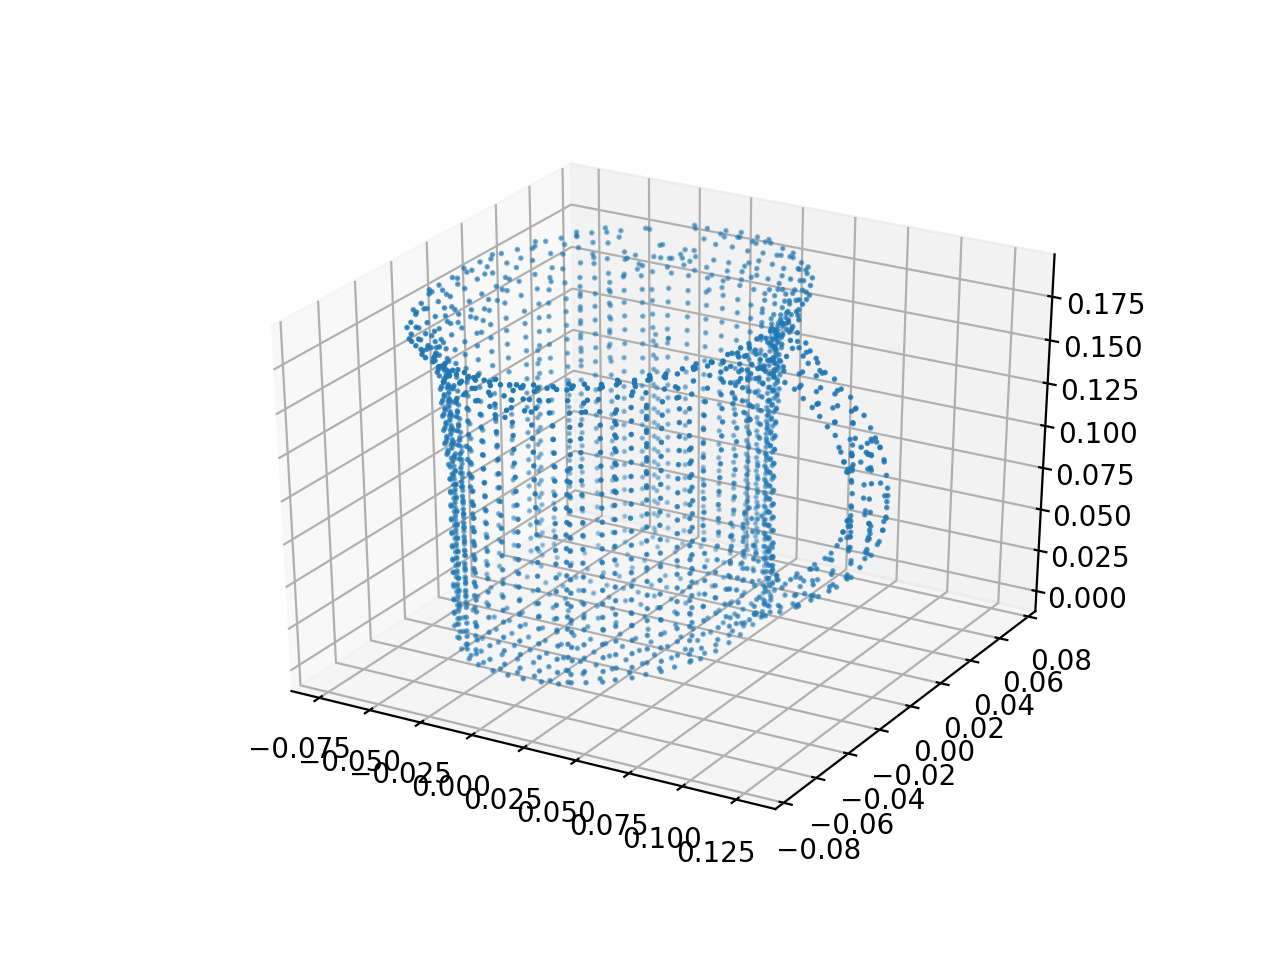
\includegraphics[width=\linewidth]{db_sample2}
    \end{subfigure}%
    \caption{Samples from Kitchen Utensil Dataset}
    \label{fig:kitchen_dataset}
\end{figure}

\subsection{Synthetic Dataset -- Multiple Holes}
For synthetic dataset, I only generate 2D point clouds so that it's simple and fast to calculate, and also easy to understand.

The first synthetic dataset contains 2D point clouds with different number of holes.
Figure ~\ref{fig:multiholes_dataset} shows some samples from this dataset.
Basically, this dataset starts from a disk-shaped point mesh.
The distance between two nearest points is 1.
Then I used different number of small holes (also have different size) to erode the disk.
The number of holes are $0, 1, 2, 3$.
The radius of holes are $2, 3, 4, 5$. 
There are totally 16 different point clouds in this dataset.

\begin{figure}[H]
    \centering
    \begin{subfigure}[h]{0.2\textwidth}
        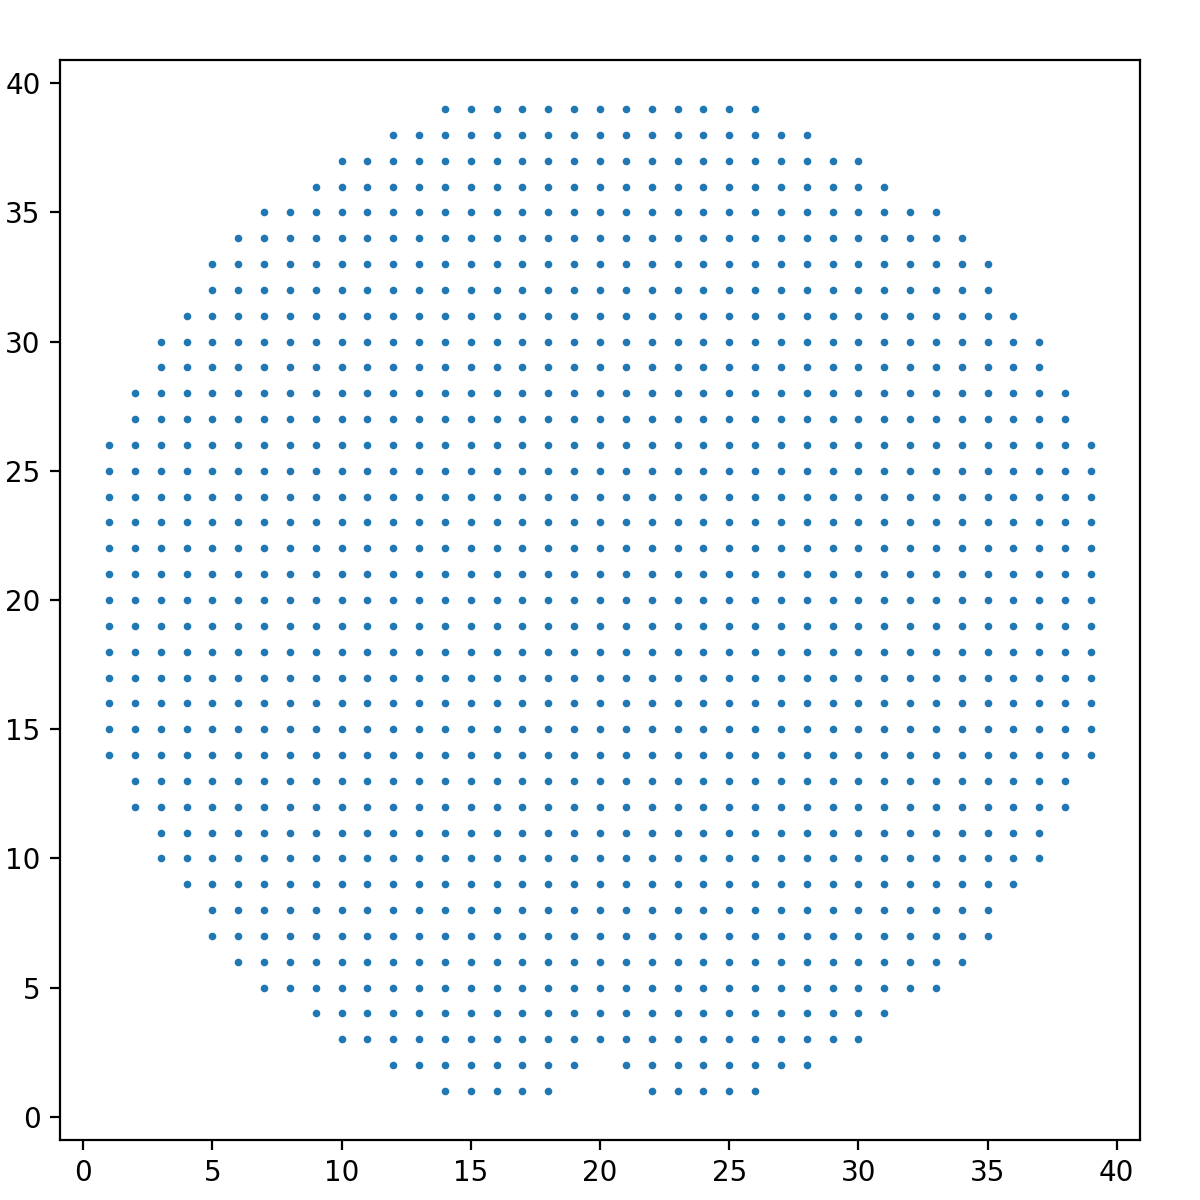
\includegraphics[width=\linewidth]{mh_1}
    \end{subfigure}
    \begin{subfigure}[h]{0.2\textwidth}
        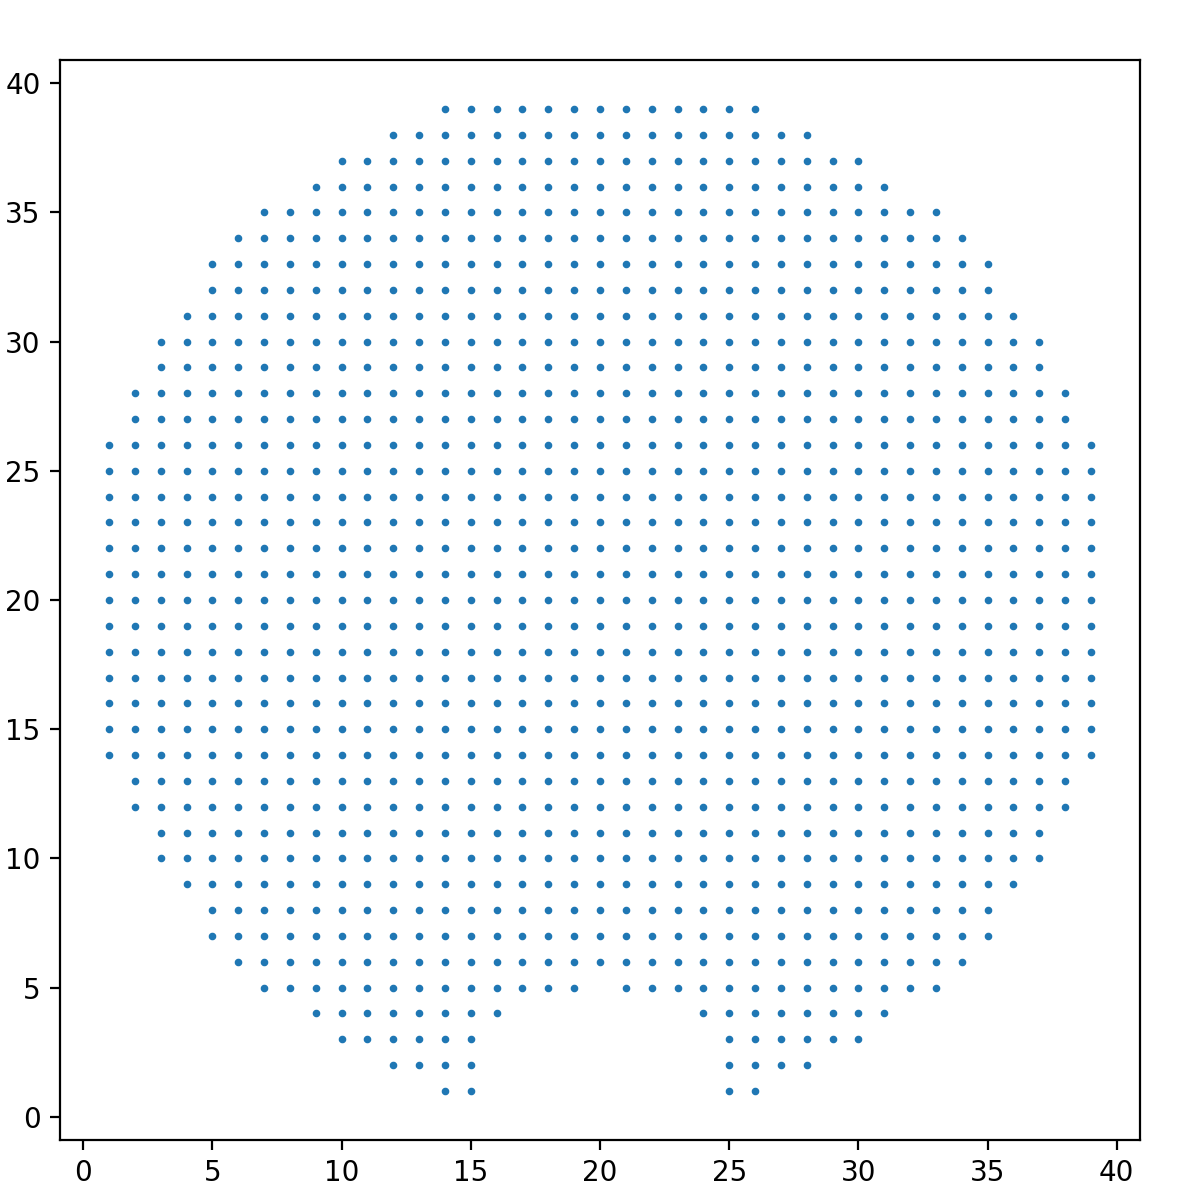
\includegraphics[width=\linewidth]{mh_2}
    \end{subfigure}%
    \begin{subfigure}[h]{0.2\textwidth}
        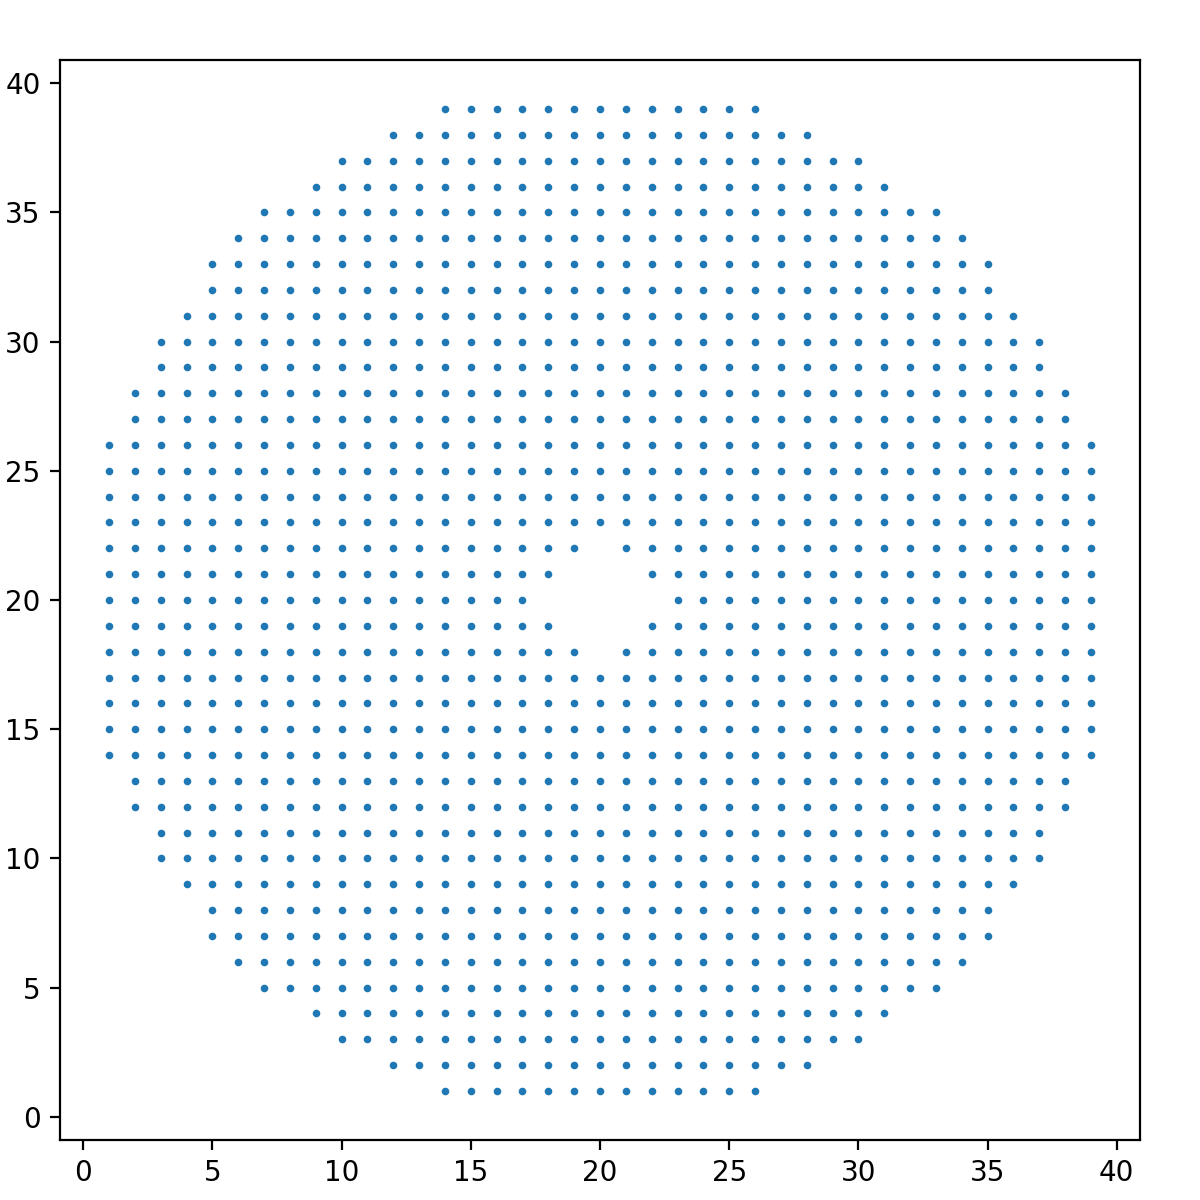
\includegraphics[width=\linewidth]{mh_3}
    \end{subfigure}%
    \begin{subfigure}[h]{0.2\textwidth}
        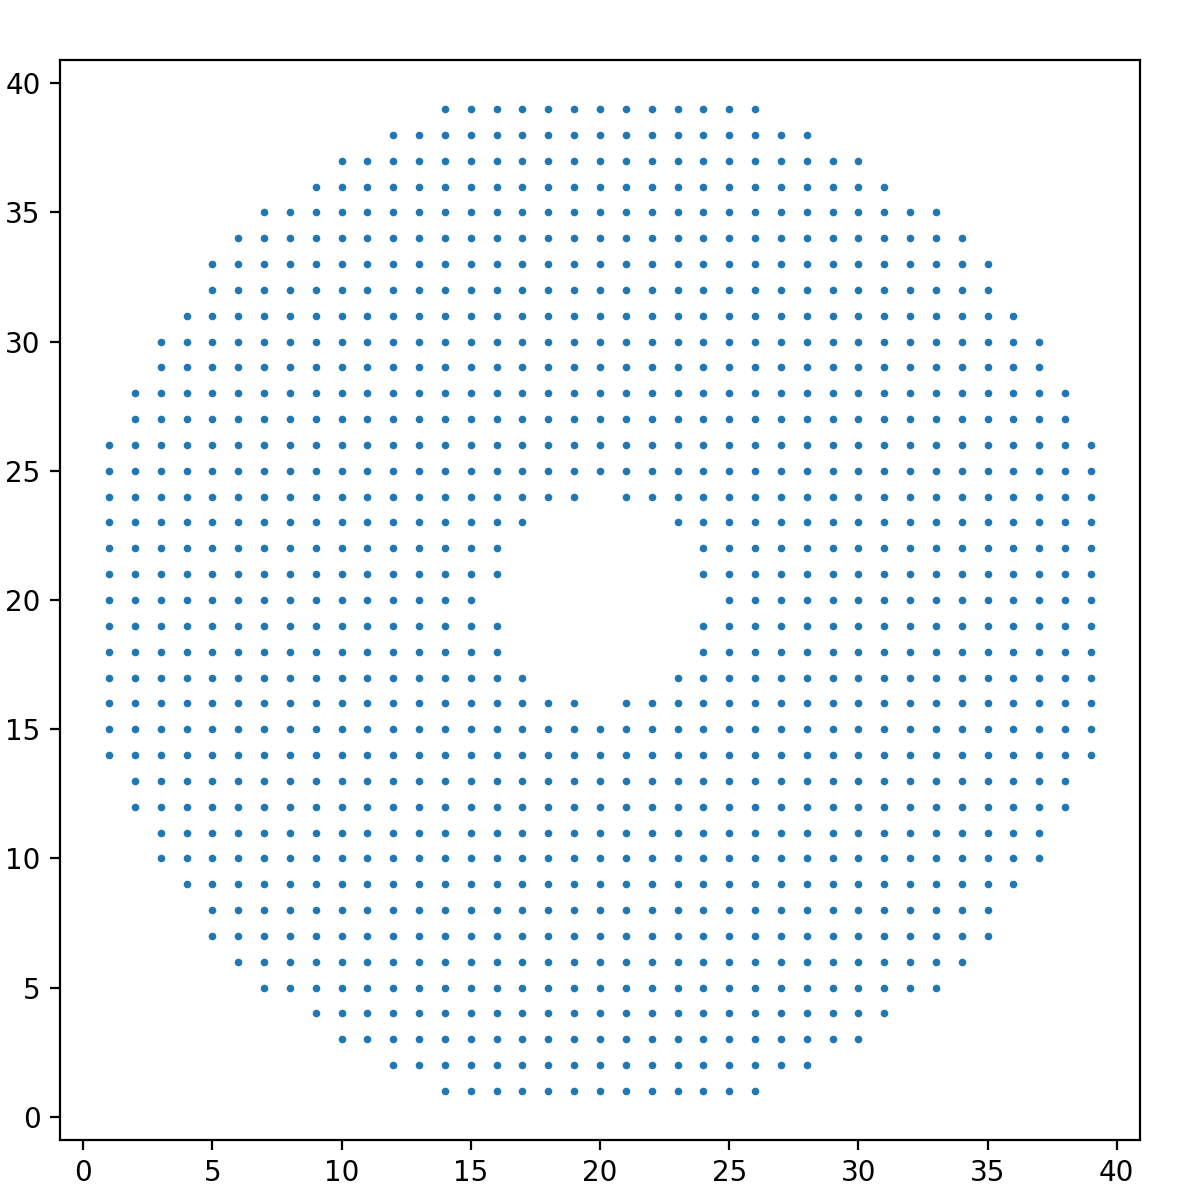
\includegraphics[width=\linewidth]{mh_4}
    \end{subfigure}%

    \begin{subfigure}[h]{0.2\textwidth}
        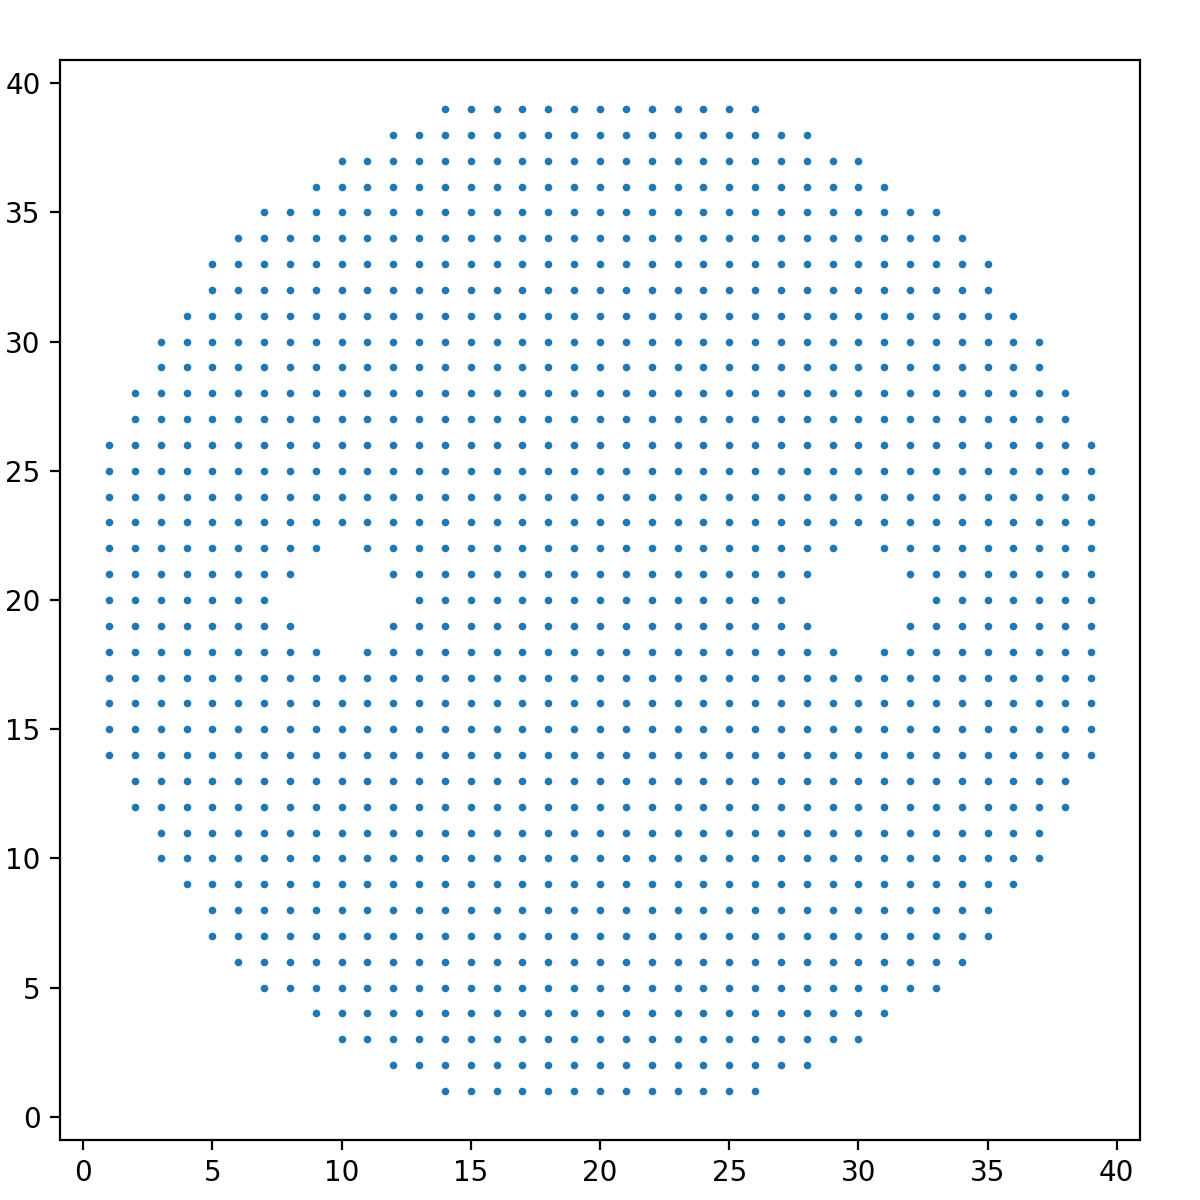
\includegraphics[width=\linewidth]{mh_5}
    \end{subfigure}
    \begin{subfigure}[h]{0.2\textwidth}
        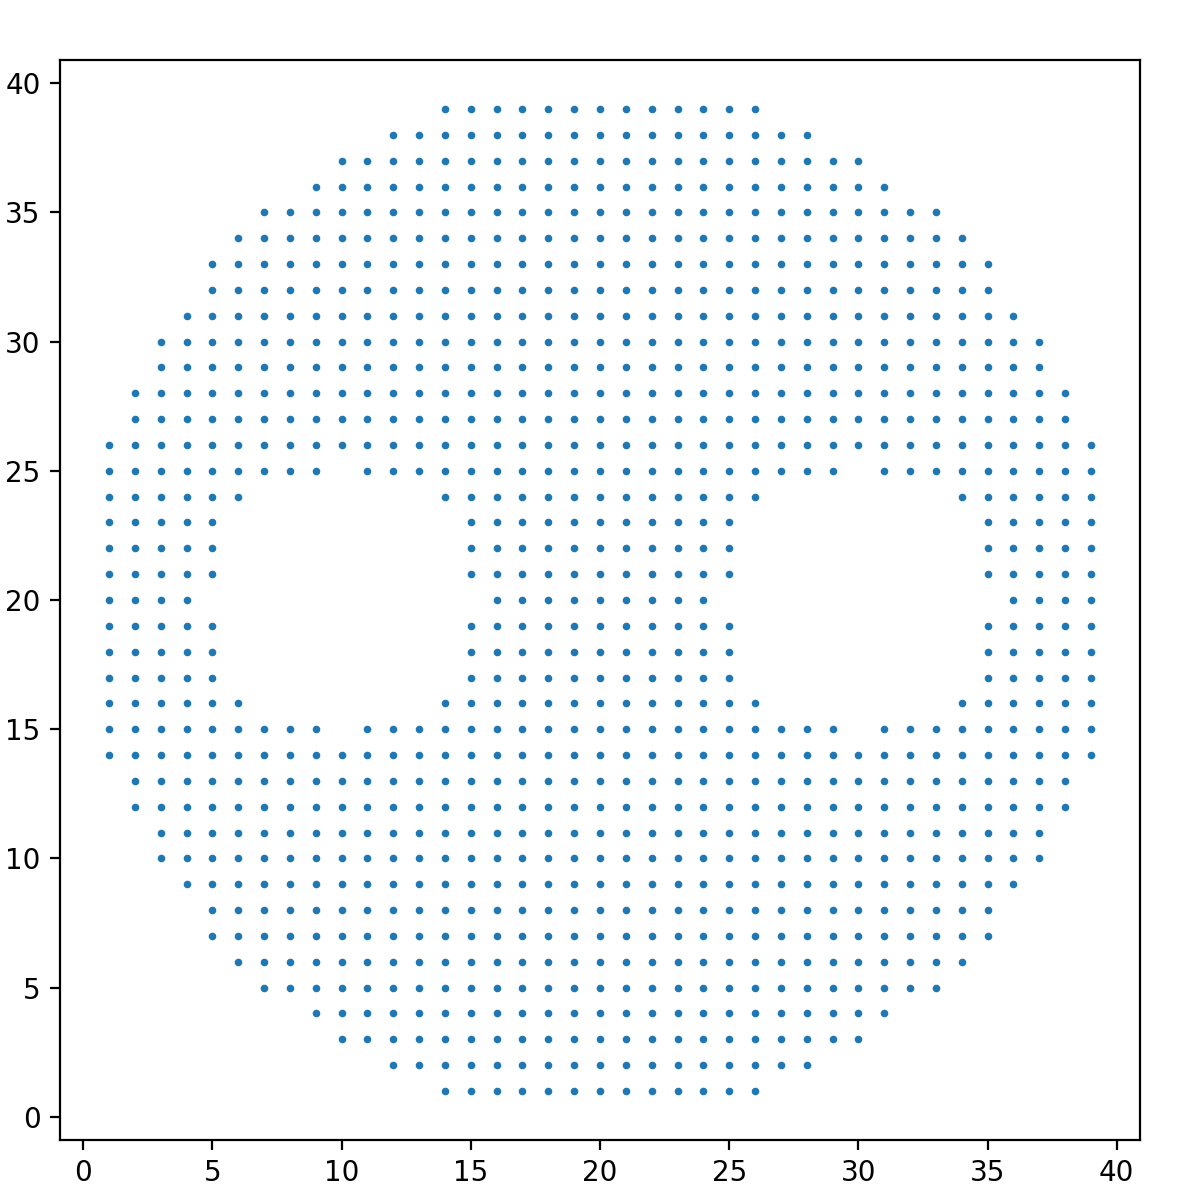
\includegraphics[width=\linewidth]{mh_6}
    \end{subfigure}%
    \begin{subfigure}[h]{0.2\textwidth}
        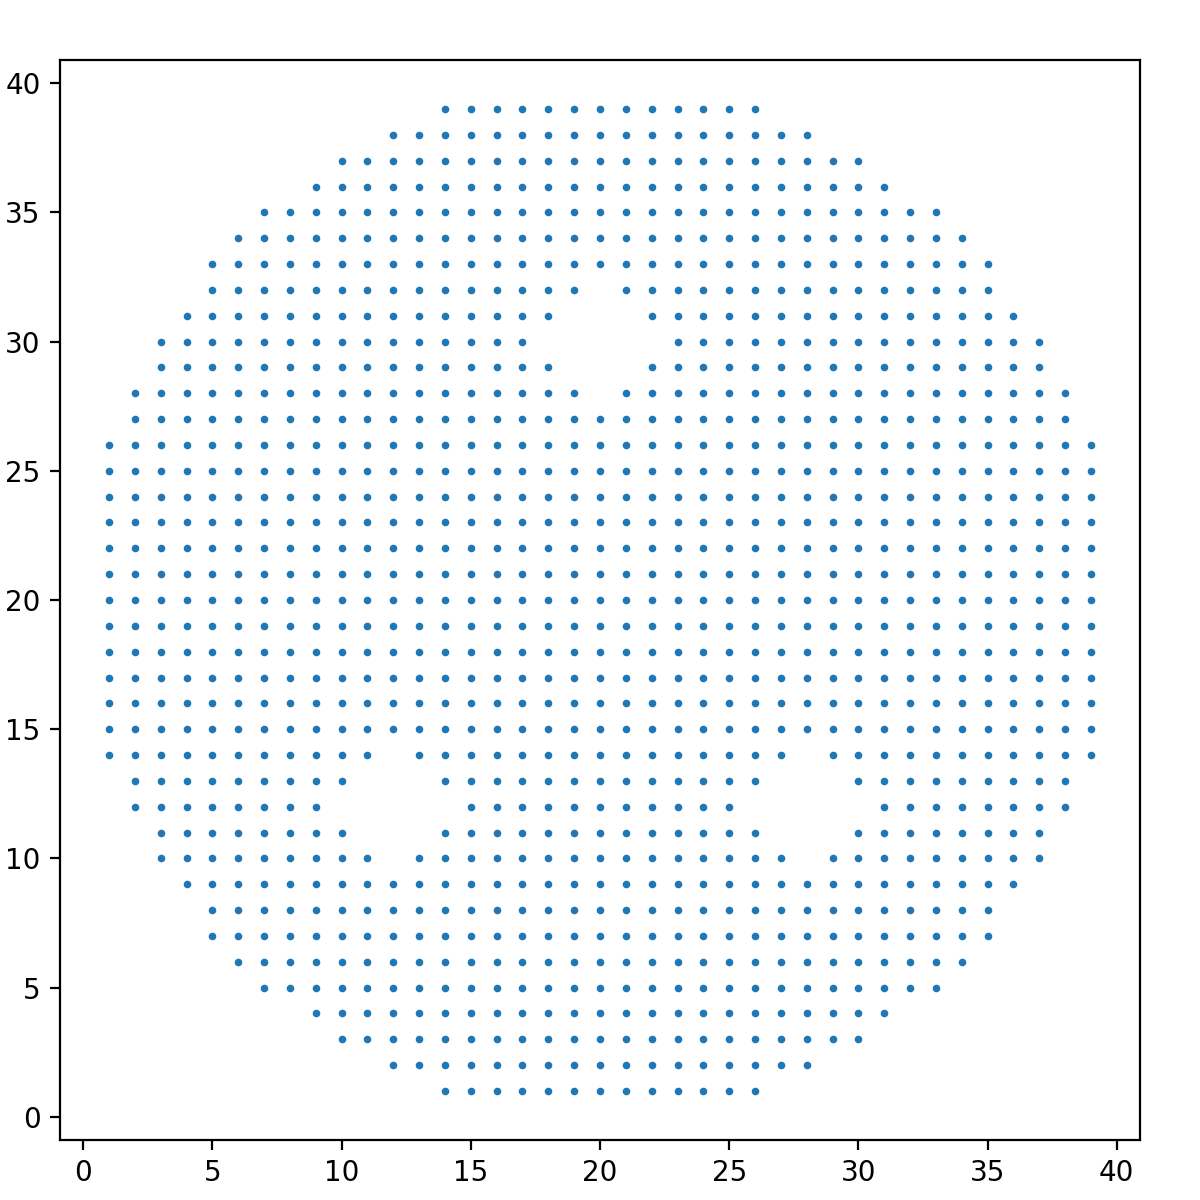
\includegraphics[width=\linewidth]{mh_7}
    \end{subfigure}%
    \begin{subfigure}[h]{0.2\textwidth}
        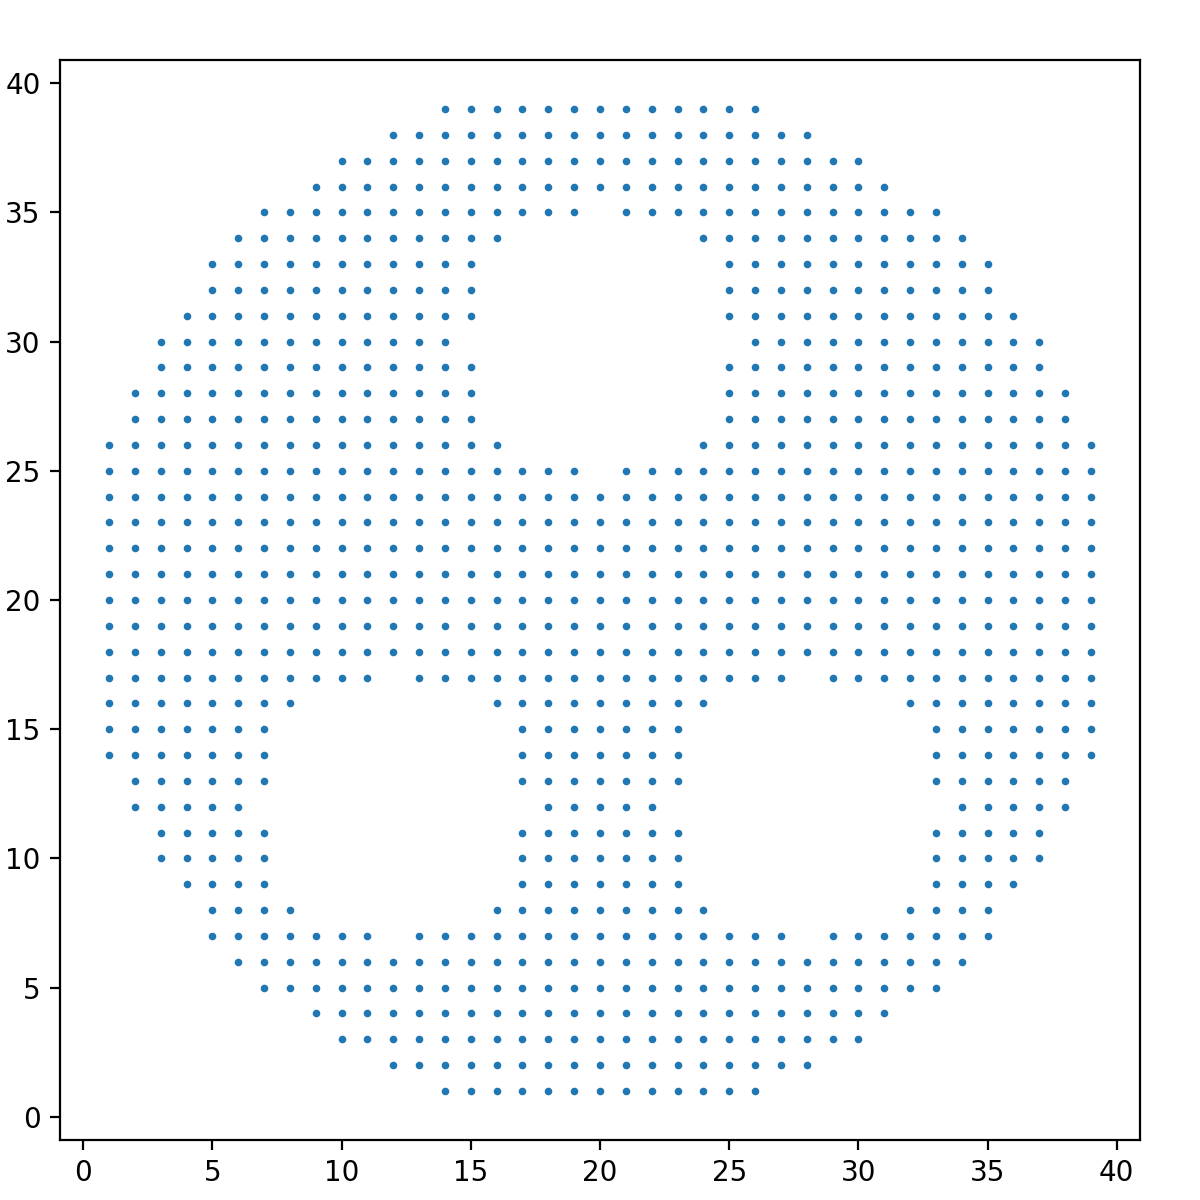
\includegraphics[width=\linewidth]{mh_8}
    \end{subfigure}%
    \caption{Synthetic Dataset: Different Number of Holes}
    \label{fig:multiholes_dataset}
\end{figure}

\subsection{Synthetic Dataset -- Multiscale}
The SMURPH kernel claims to be capable of doing multiresolution analysis.
So I designed this dataset to evaluate this ability.
Figure ~\ref{fig:multiscale_dataset} shows a few samples.
The dataset basically have two shapes of data: ``O" and ``$\infty$".
Each shape could be consist of solid ribbons, or ribbons with small holes.
These four point clouds, as Figure ~\ref{fig:multiscale_dataset} shows, forms a set.
There are 3 sets in this dataset with size $40 \times 40$, $25 \times 25$, and $8 \times 8$.

\begin{figure}[H]
    \centering
    \begin{subfigure}[h]{0.2\textwidth}
        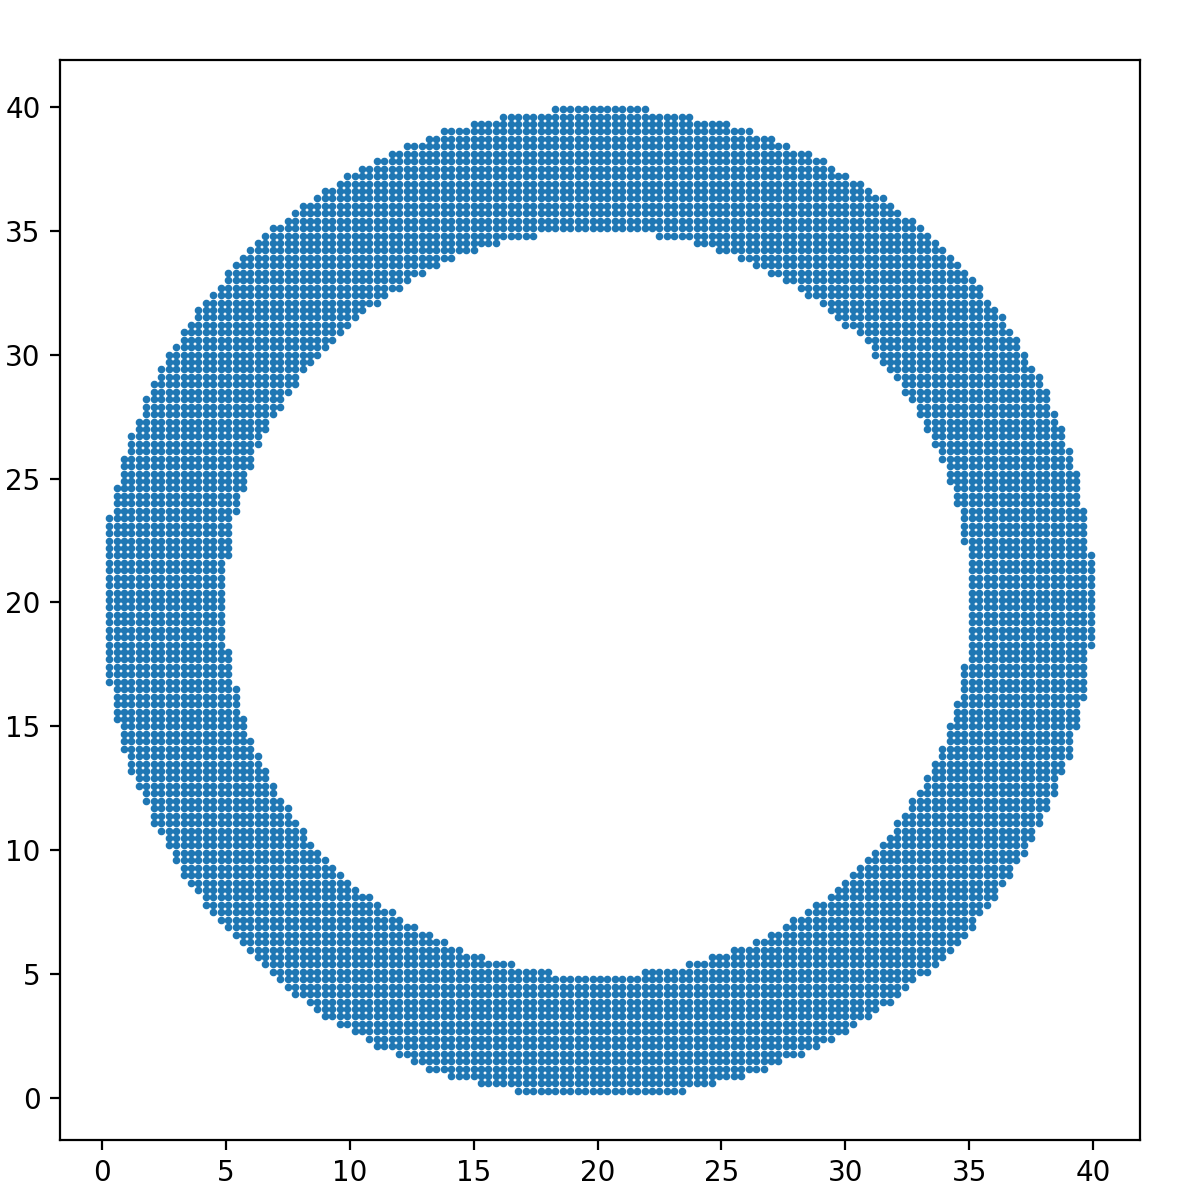
\includegraphics[width=\linewidth]{ms_1}
    \end{subfigure}
    \begin{subfigure}[h]{0.2\textwidth}
        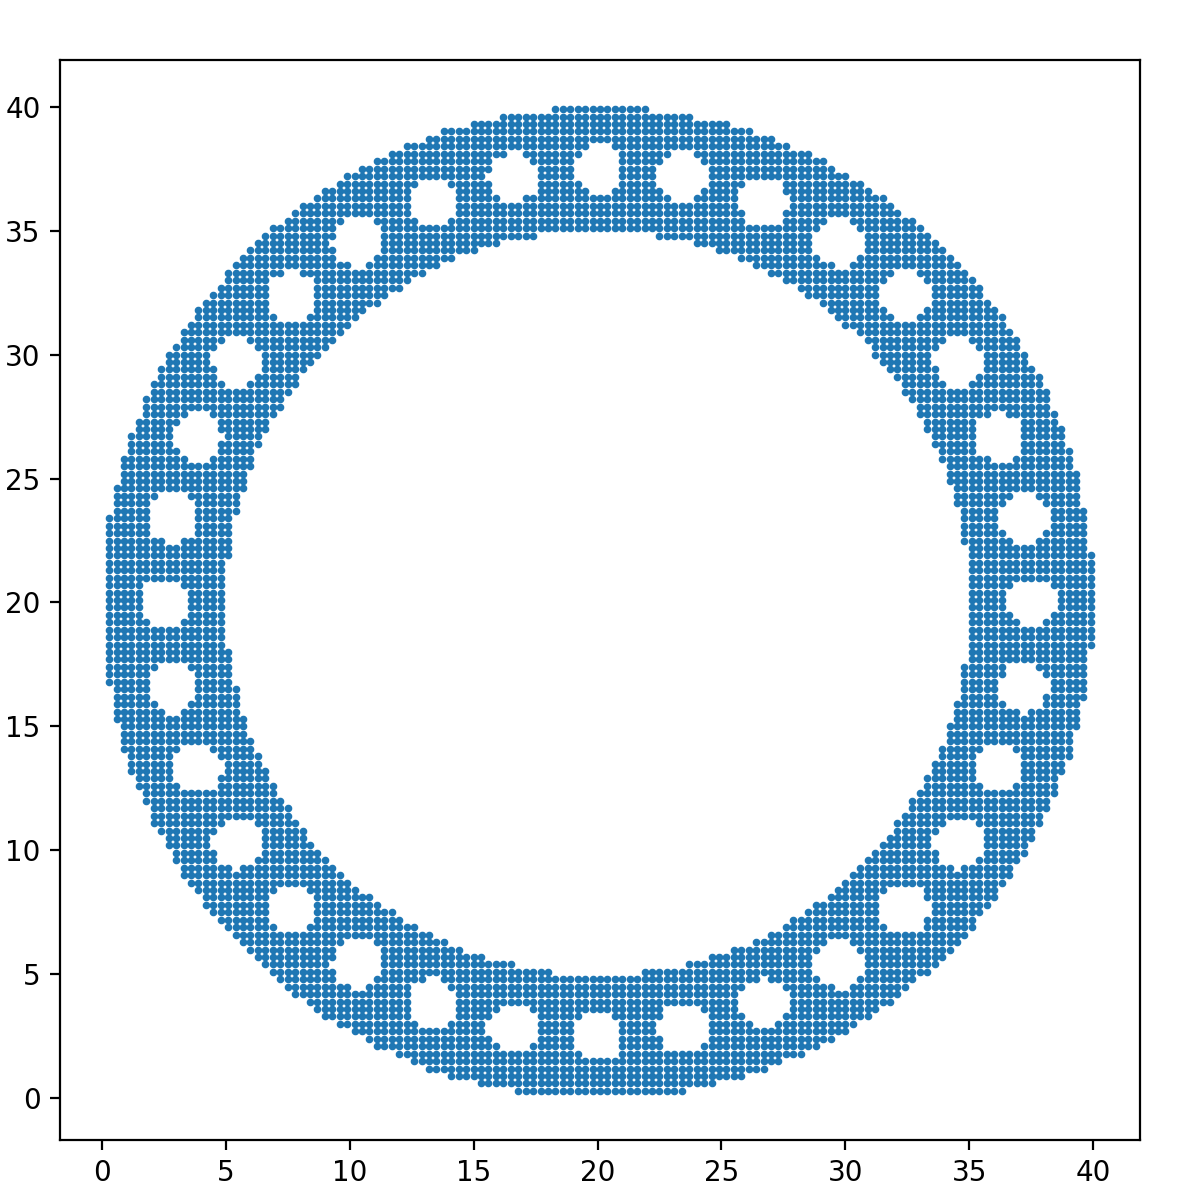
\includegraphics[width=\linewidth]{ms_2}
    \end{subfigure}%
    \begin{subfigure}[h]{0.2\textwidth}
        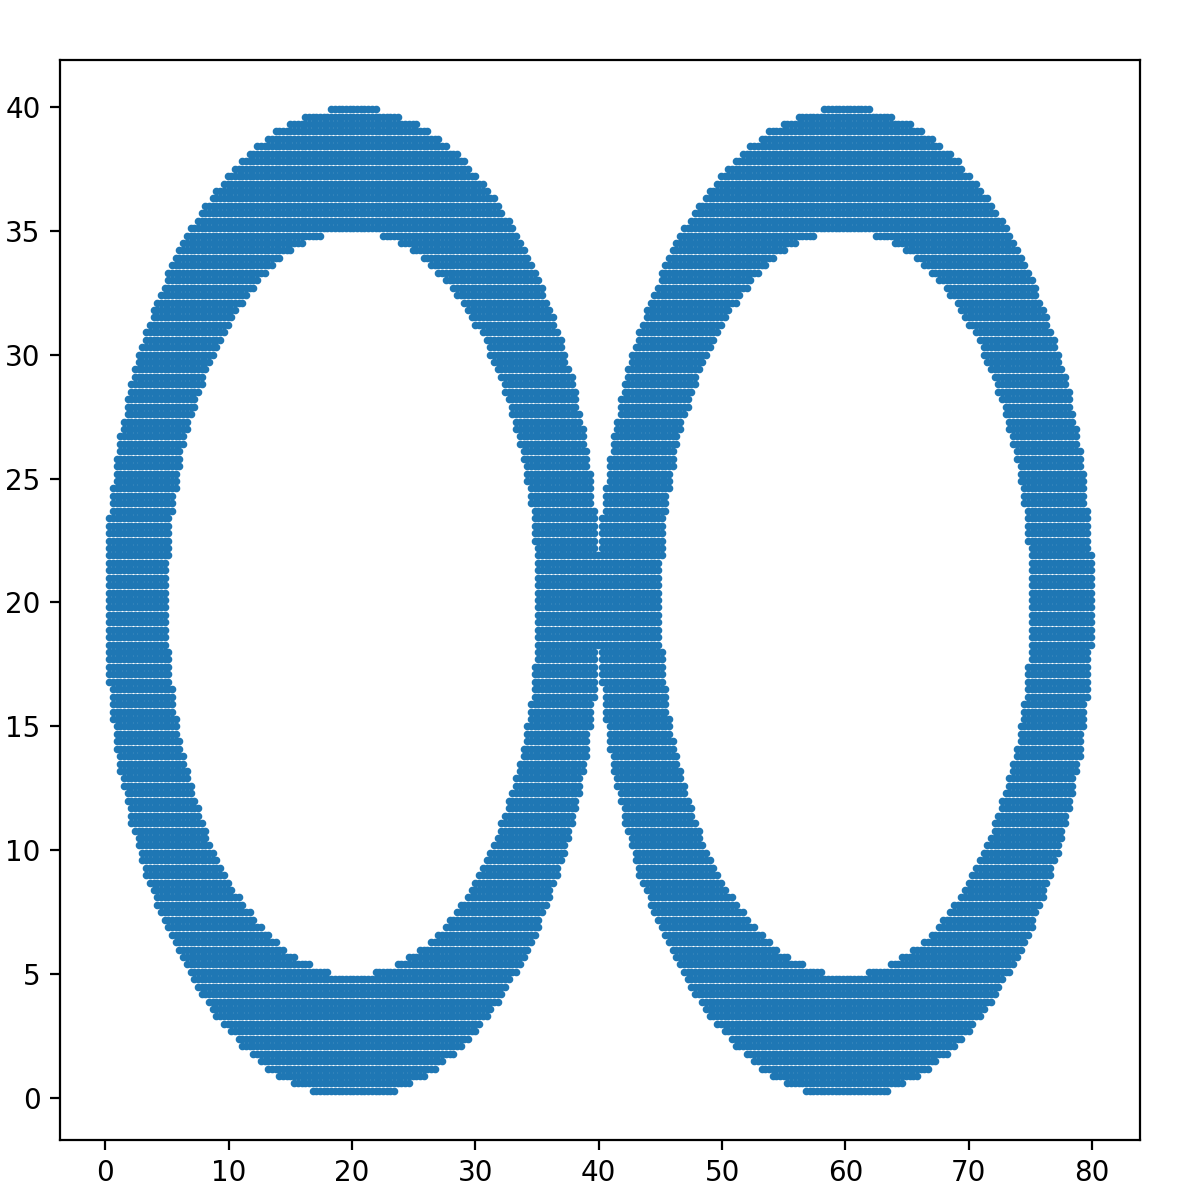
\includegraphics[width=\linewidth]{ms_3}
    \end{subfigure}%
    \begin{subfigure}[h]{0.2\textwidth}
        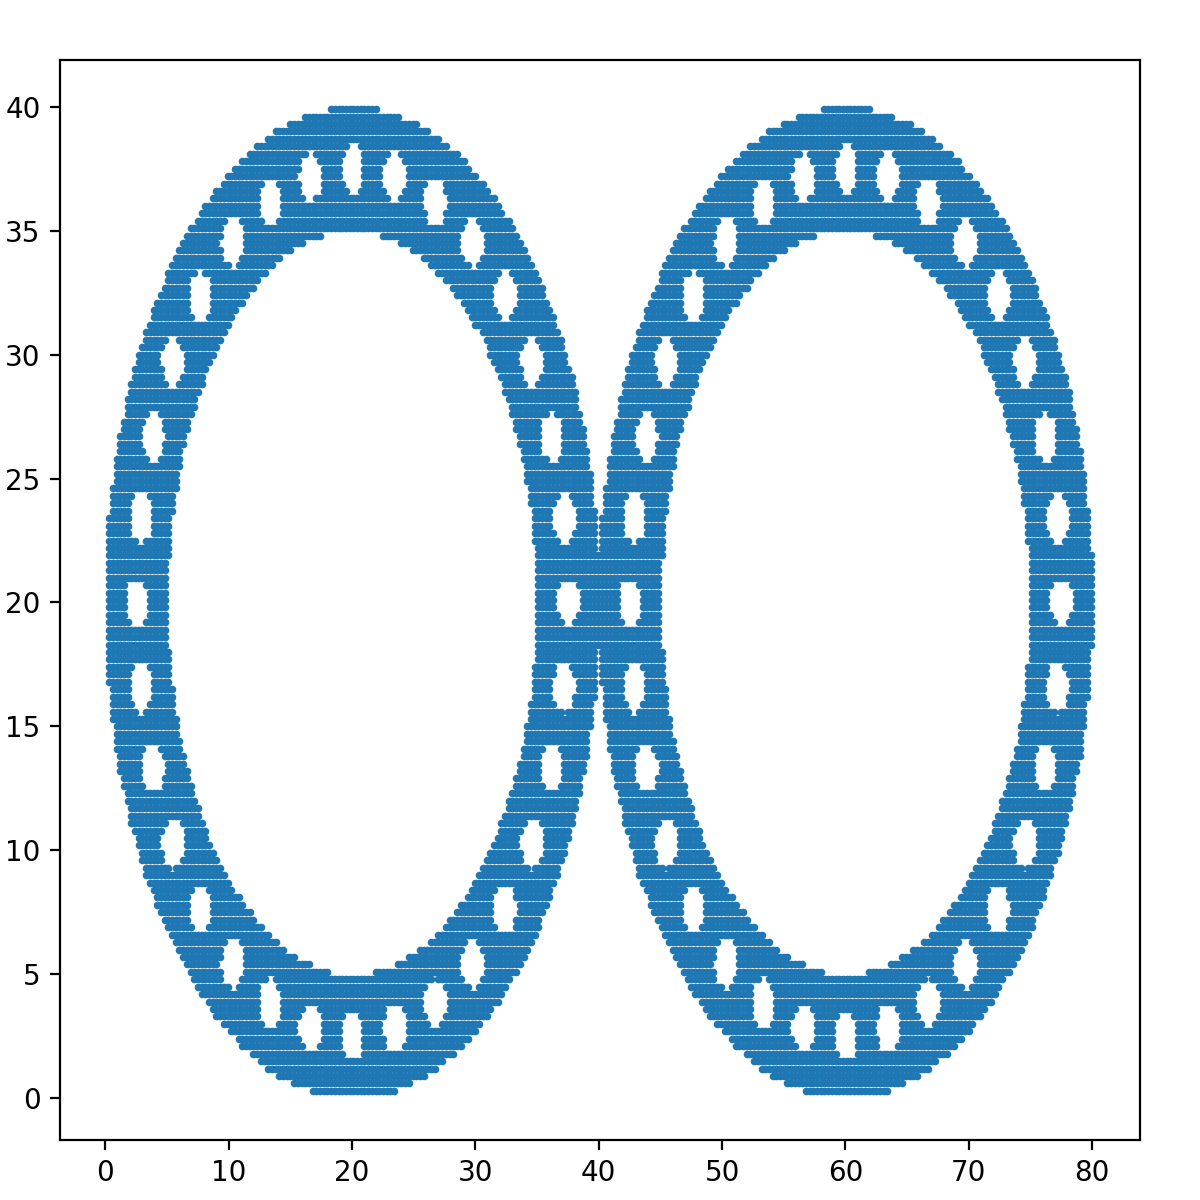
\includegraphics[width=\linewidth]{ms_4}
    \end{subfigure}%
    \caption{Synthetic Dataset: Different Scale of Holes}
    \label{fig:multiscale_dataset}
\end{figure}

\section{Experimental Results}

\subsection{Kitchen Utensil Dataset}

First, in order to validate my implementation of SMURPH kernel, I compared the kernel PCA result
with the result given in the original paper. 
One thing to notice is that the parameters I used in my implementation is slightly different.
This is due to the computation limitation.
Specifically, in the original paper, they used a radius of $r = 0.1$, $m = 20$ centers per point cloud, $s = 1$ samples per center, and a budget of $b = 350$ points per sample.
In my experiment, I used a radius of $r = 0.1$, $m = 10$ centers per point cloud, $s = 1$ samples per center, and a budget of $b = 100$ points per sample.
The comparison is shown in Figure ~\ref{fig:smurph_compare}.
As we can see, the overall distribution of my implementation is very close to the result from original paper.

\begin{figure}[H]
    \centering
    \begin{subfigure}[h]{0.4\textwidth}
        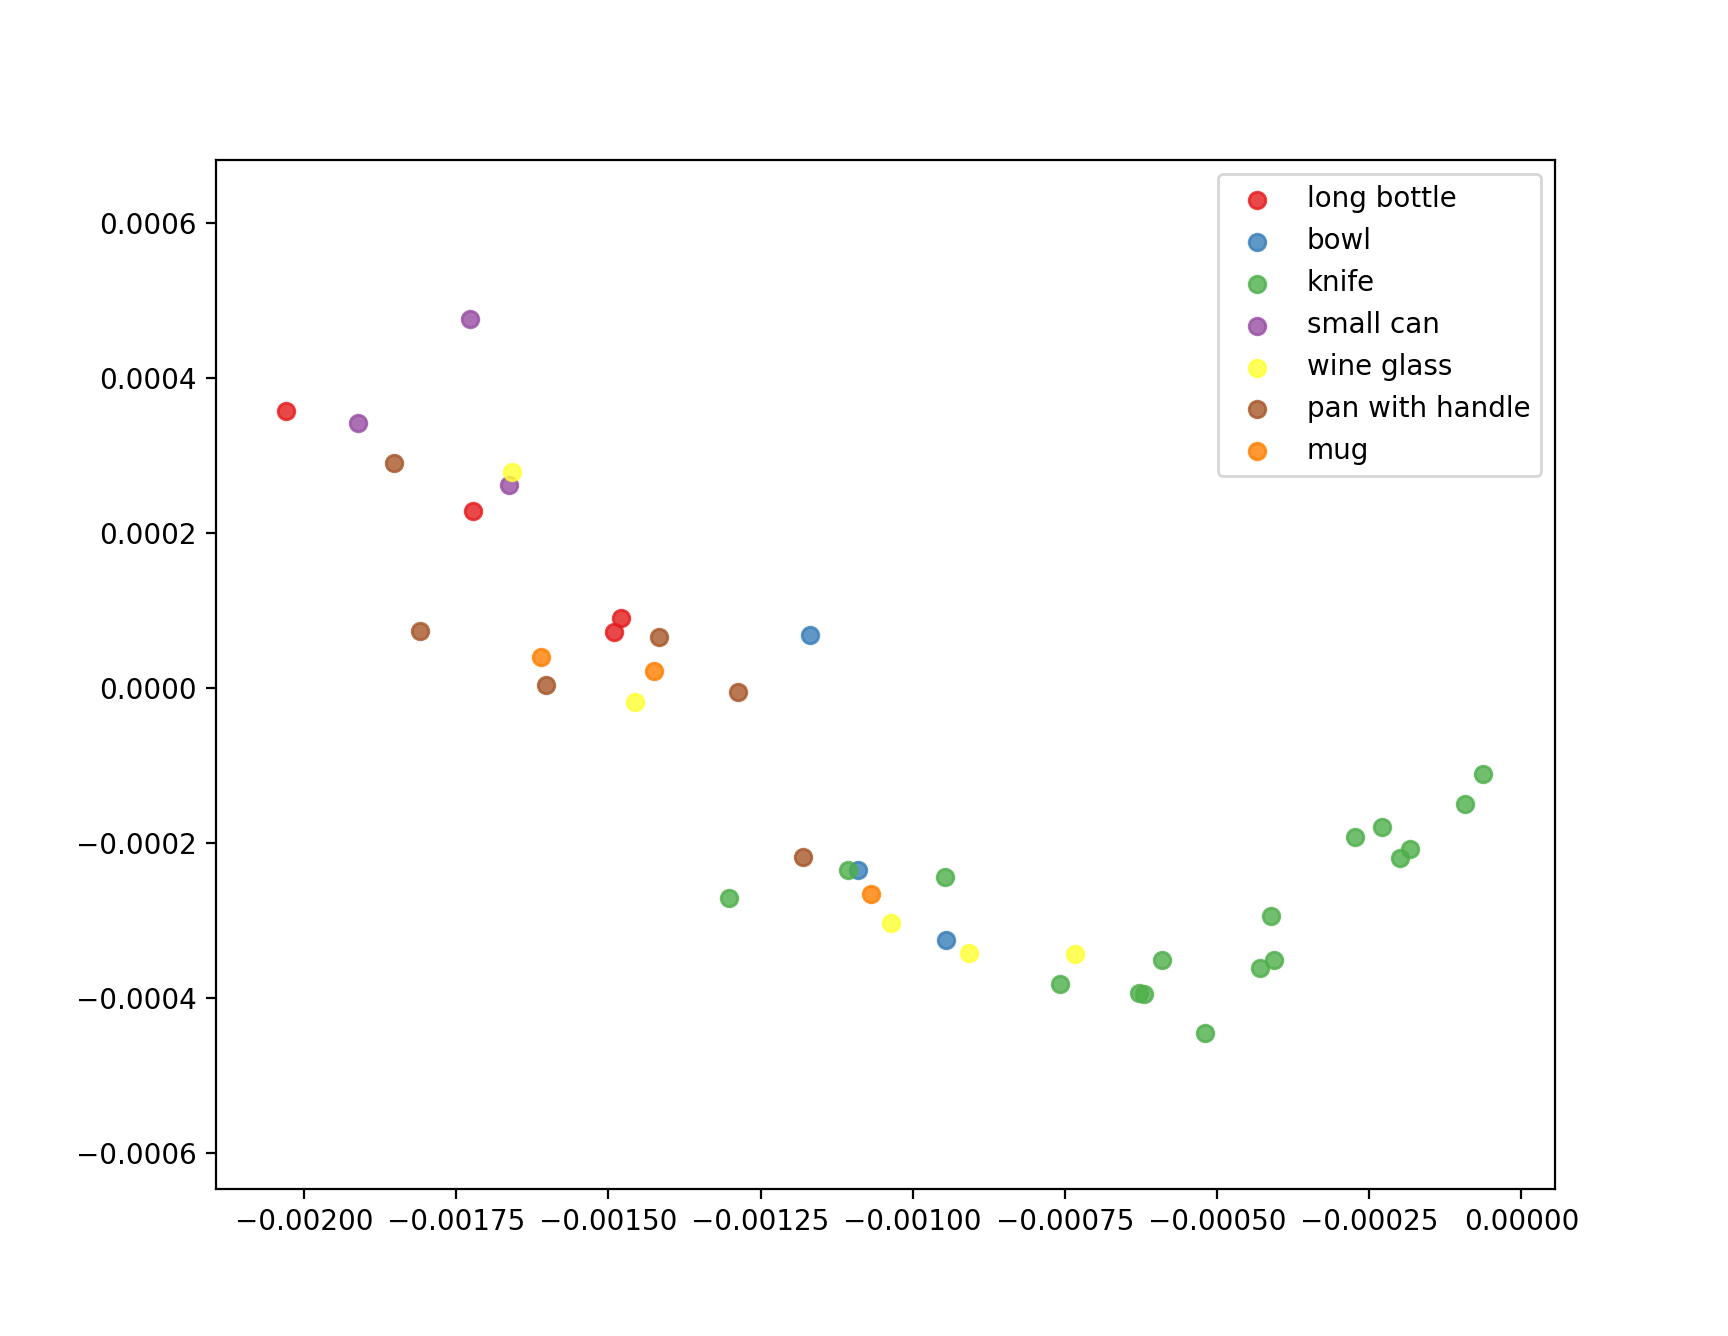
\includegraphics[width=\linewidth]{DB_smurf}
        \caption{My implementation}
    \end{subfigure}
    \begin{subfigure}[h]{0.37\textwidth}
        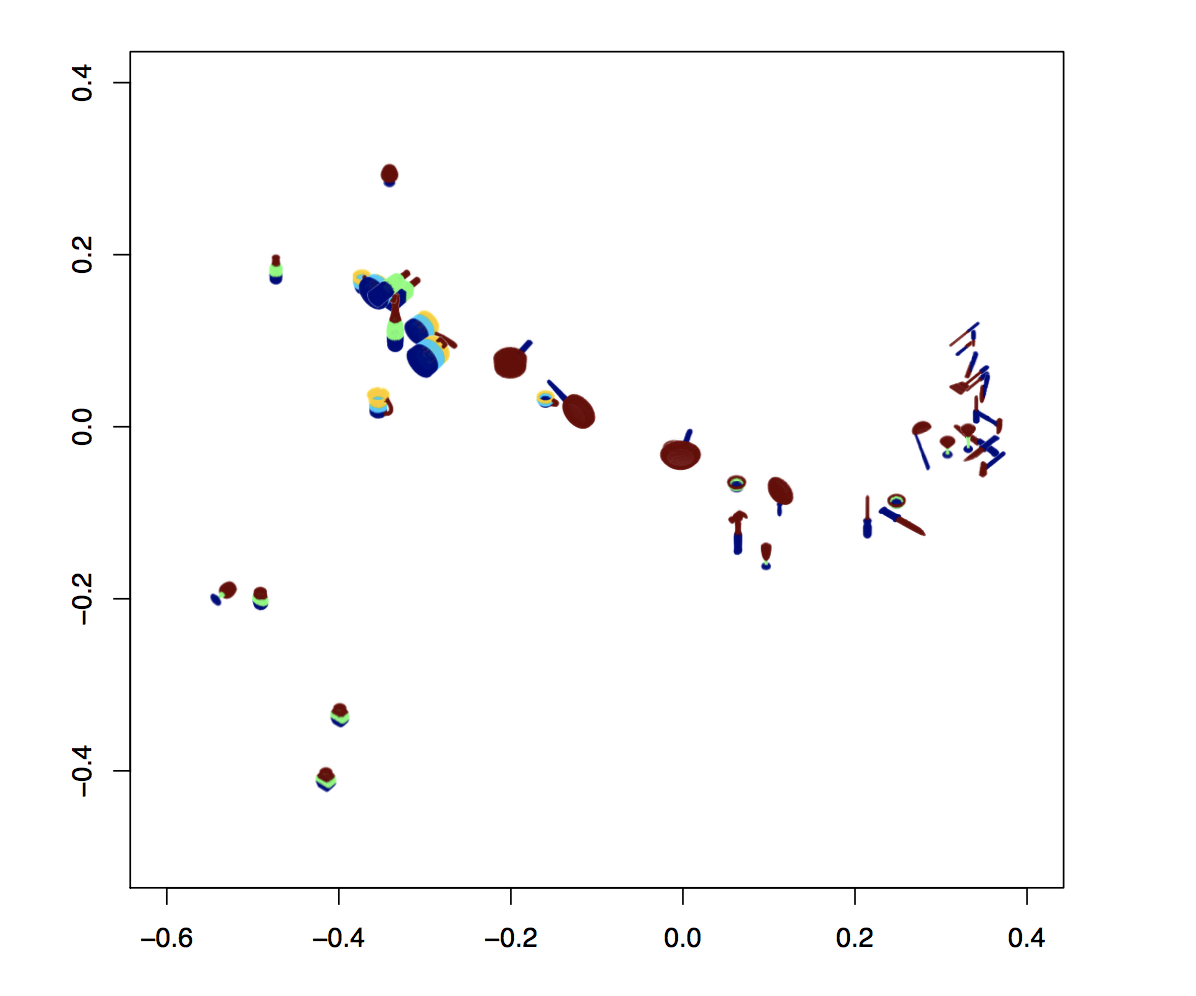
\includegraphics[width=\linewidth]{original_smurph}
        \caption{Result from original paper}
    \end{subfigure}%
    \caption{SMURPH kernel PCA results for Kitchen Utensil Dataset}
    \label{fig:smurph_compare}
\end{figure}



\begin{figure}[H]
    \centering
    \begin{subfigure}[h]{0.33\textwidth}
        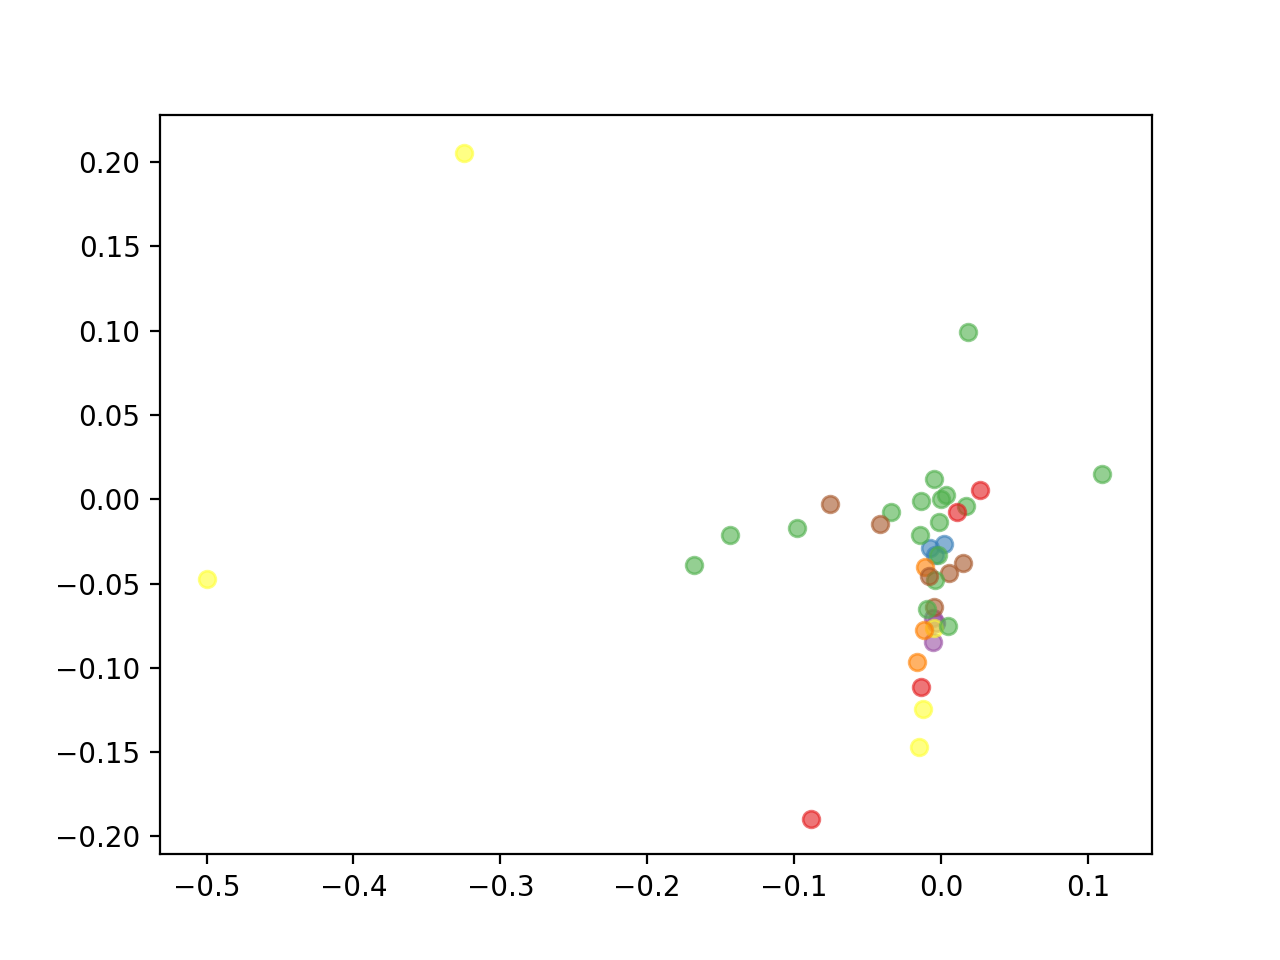
\includegraphics[width=\linewidth]{DB_linear}
        \caption{Linear Kernel}
    \end{subfigure}
    \begin{subfigure}[h]{0.33\textwidth}
        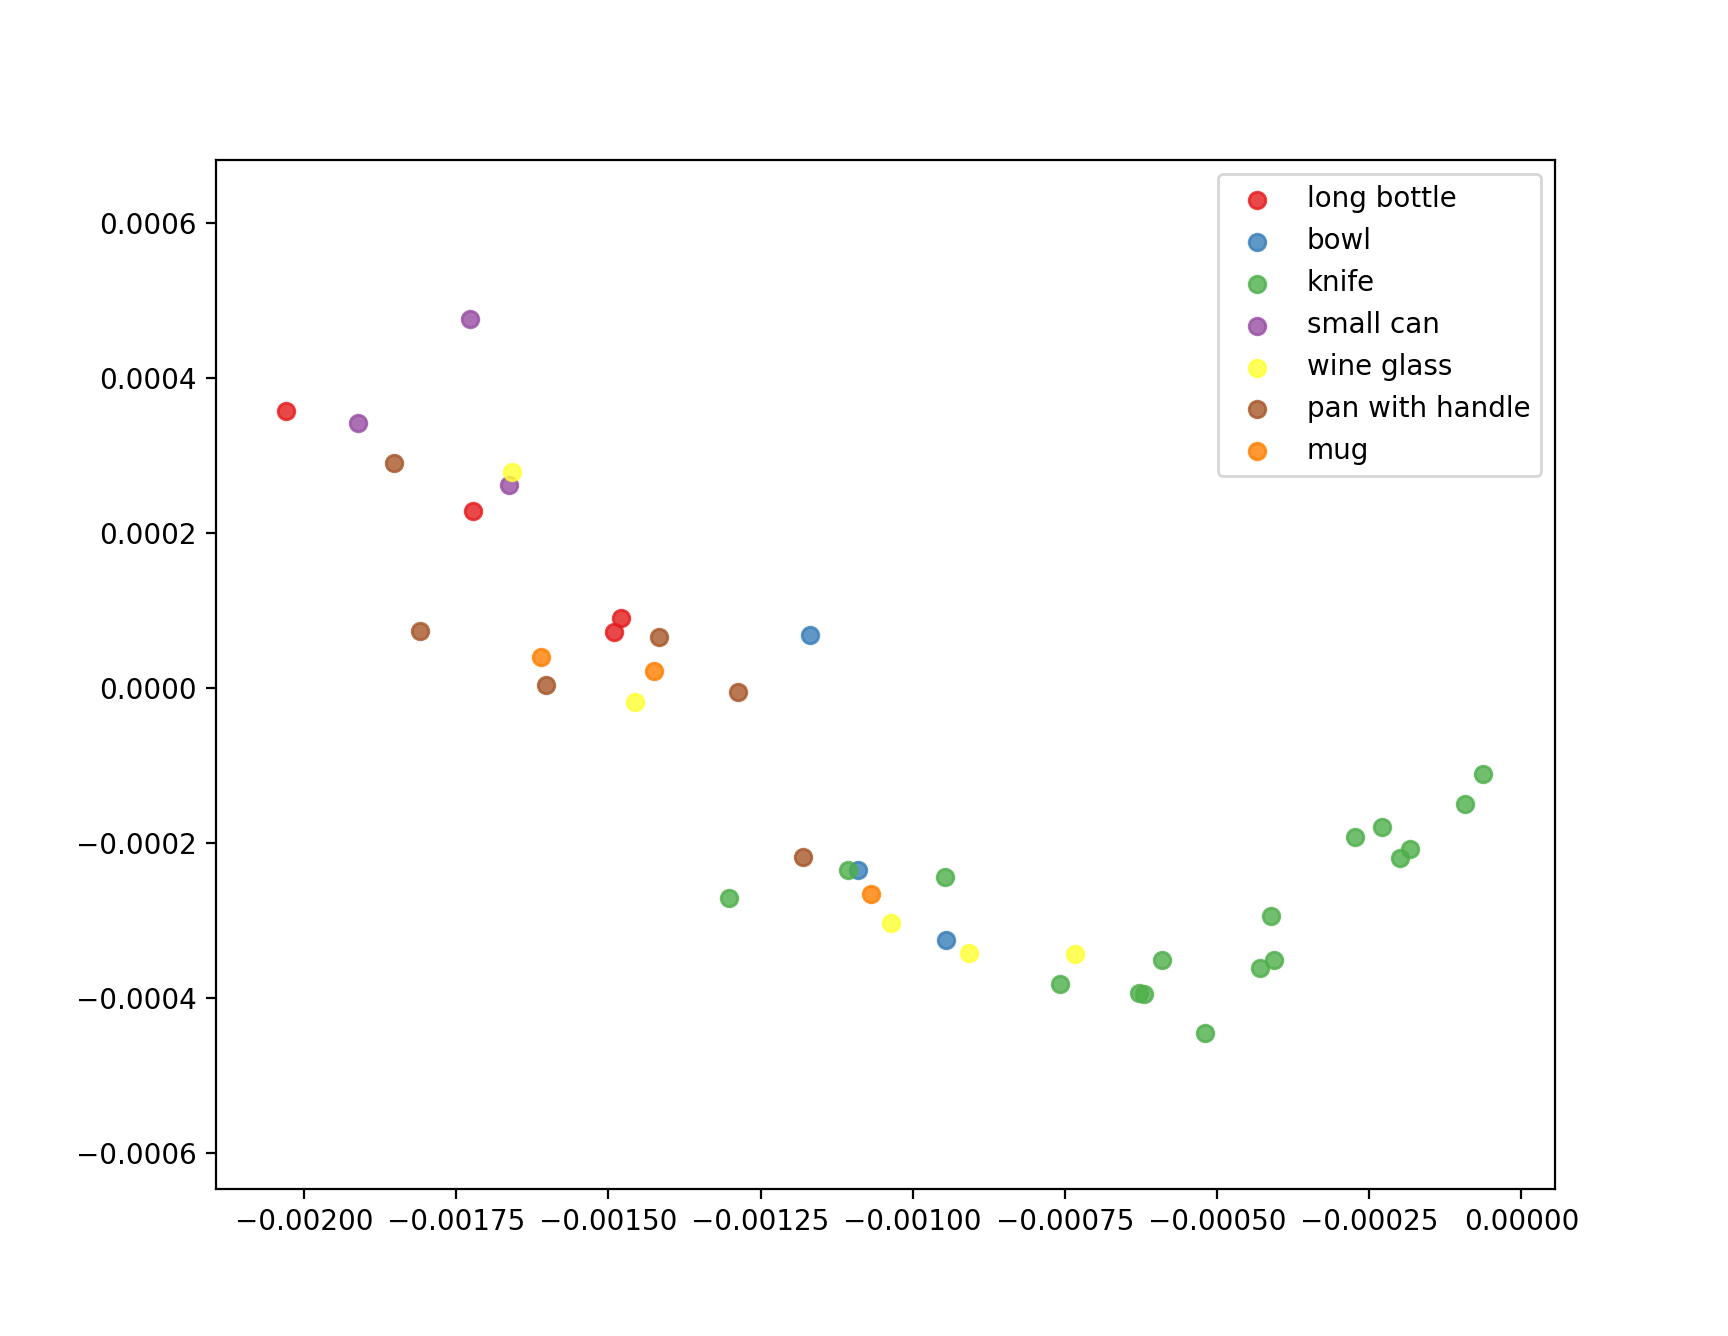
\includegraphics[width=\linewidth]{DB_smurf}
        \caption{SMURPH Kernel}
    \end{subfigure}%
    \begin{subfigure}[h]{0.33\textwidth}
        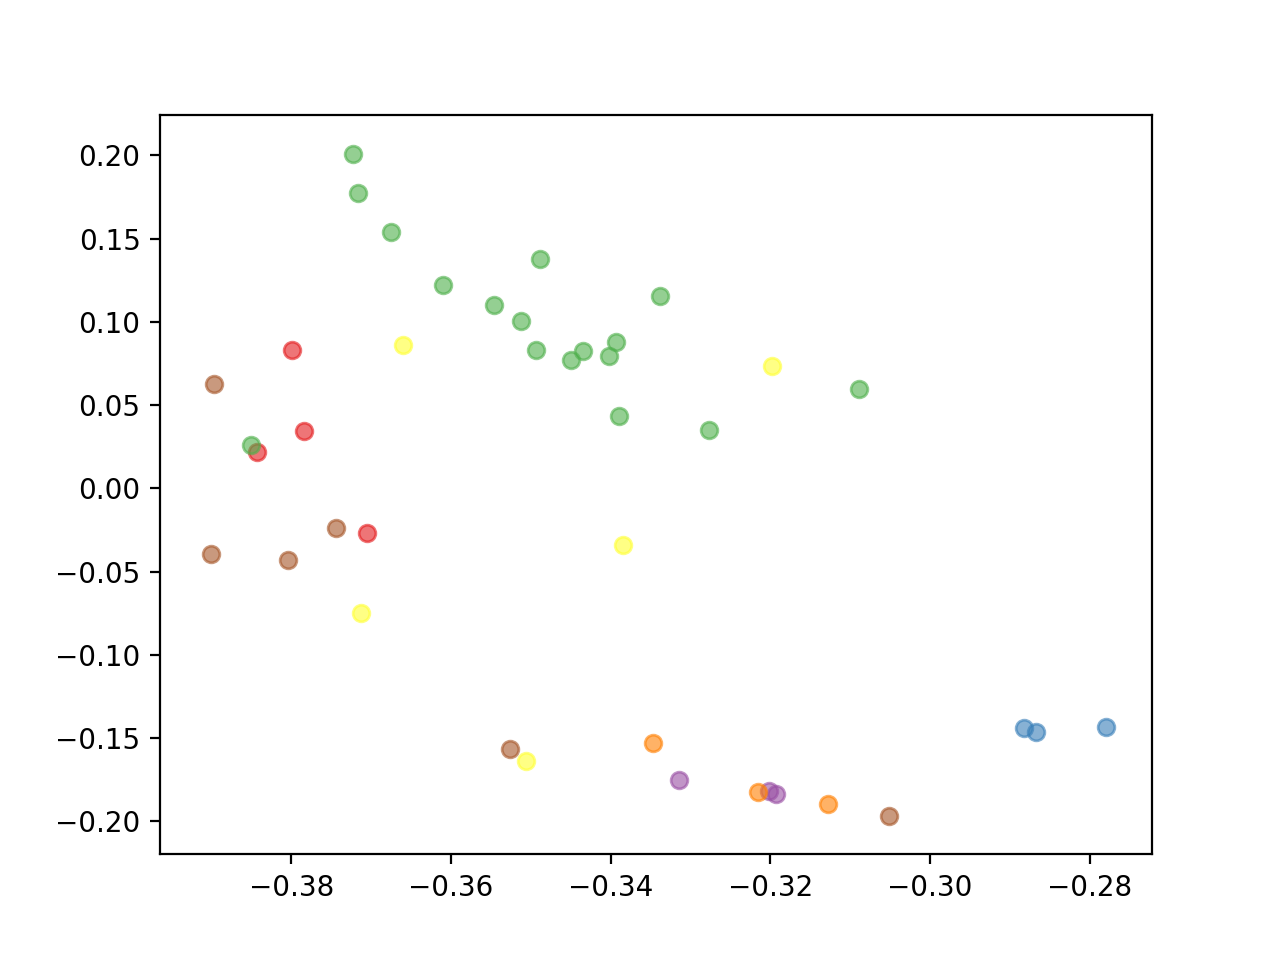
\includegraphics[width=\linewidth]{DB_hod}
        \caption{HOD Kernel}
    \end{subfigure}%
    \caption{Kernel PCA results for Kitchen Utensil Dataset}
\end{figure}

\subsection{Synthetic Dataset -- Multiple Holes}

\begin{figure}[H]
    \centering
    \begin{subfigure}[h]{0.33\textwidth}
        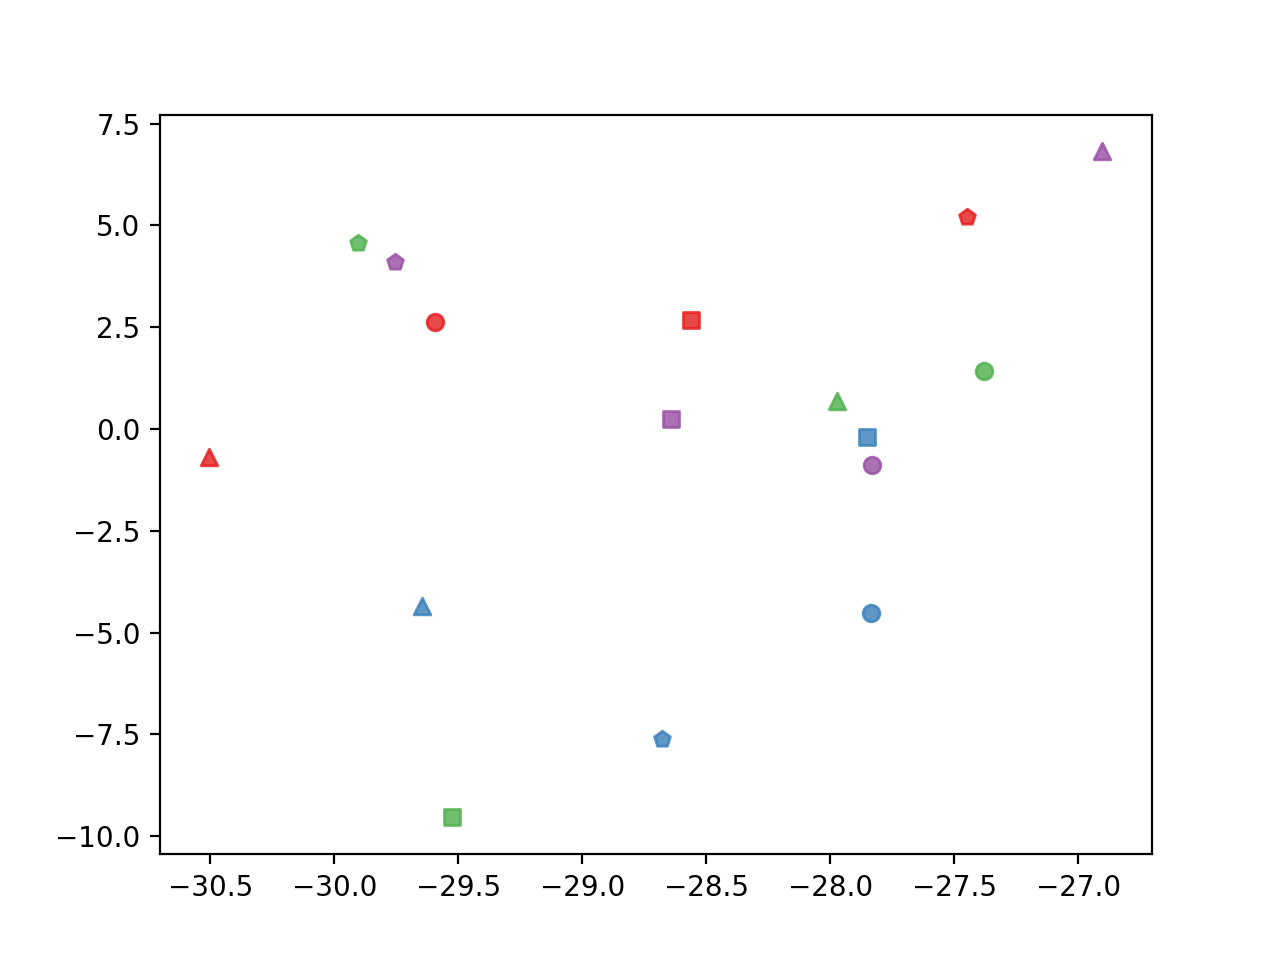
\includegraphics[width=\linewidth]{mh_linear}
        \caption{Linear Kernel}
    \end{subfigure}
    \begin{subfigure}[h]{0.33\textwidth}
        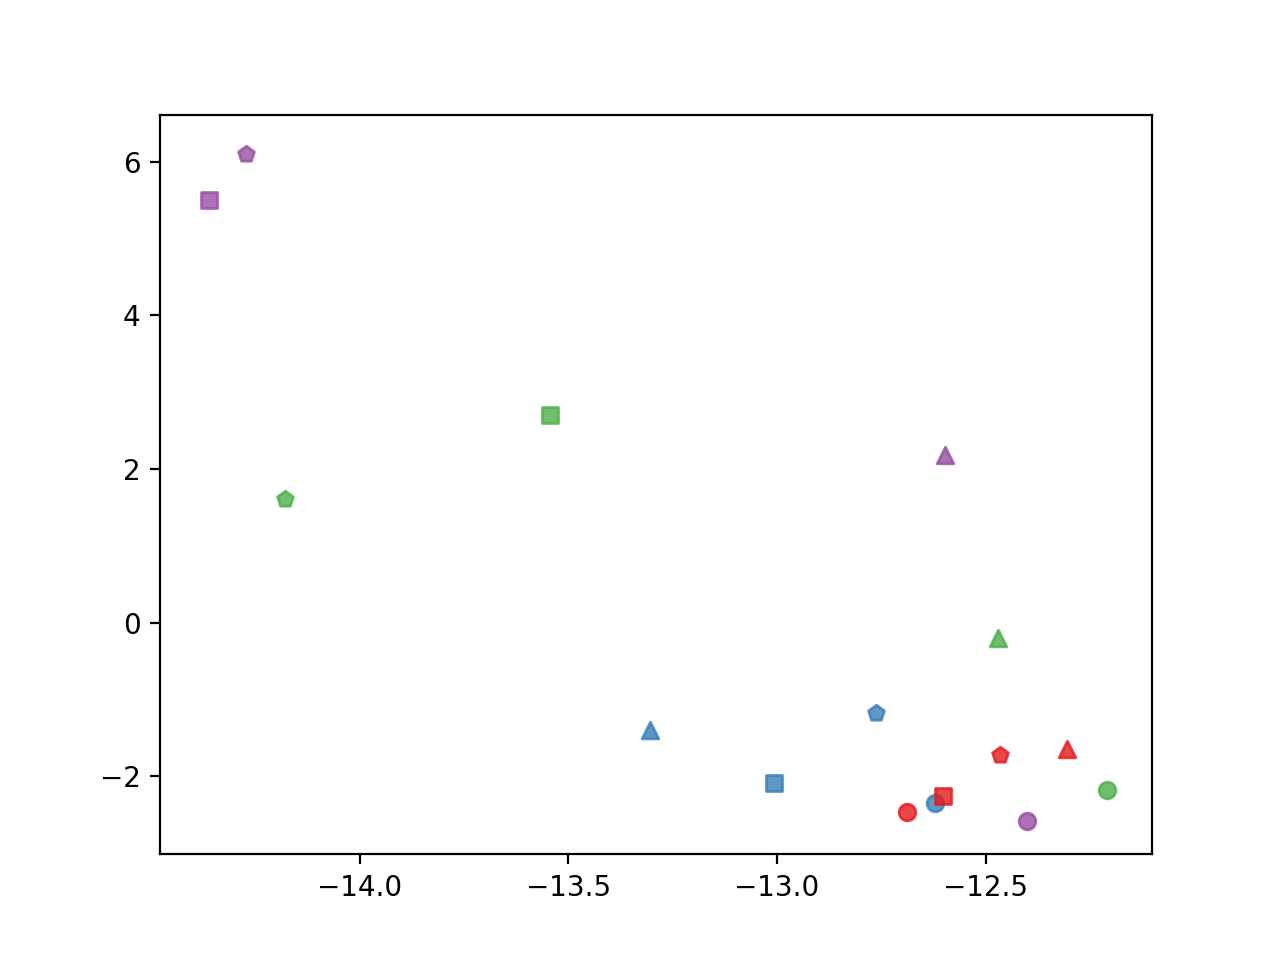
\includegraphics[width=\linewidth]{mh_smurf}
        \caption{SMURPH Kernel}
    \end{subfigure}%
    \begin{subfigure}[h]{0.33\textwidth}
        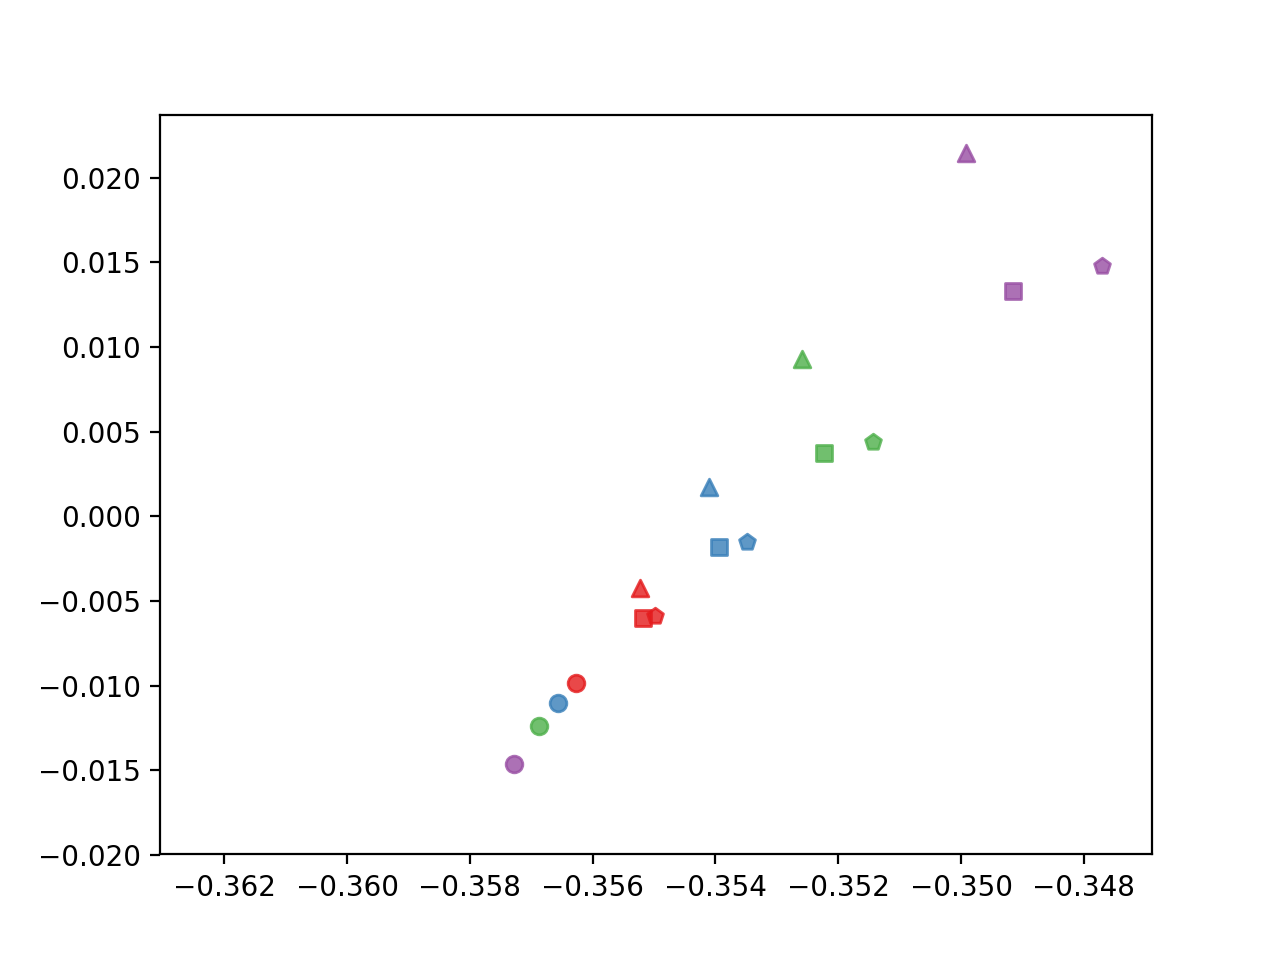
\includegraphics[width=\linewidth]{mh_hod}
        \caption{HOD Kernel}
    \end{subfigure}%
    \caption{Kernel PCA results for Synthetic Multiholes Dataset}
\end{figure}

\subsection{Synthetic Dataset -- Multiscale}

\begin{figure}[H]
    \centering
    \begin{subfigure}[h]{0.3\textwidth}
        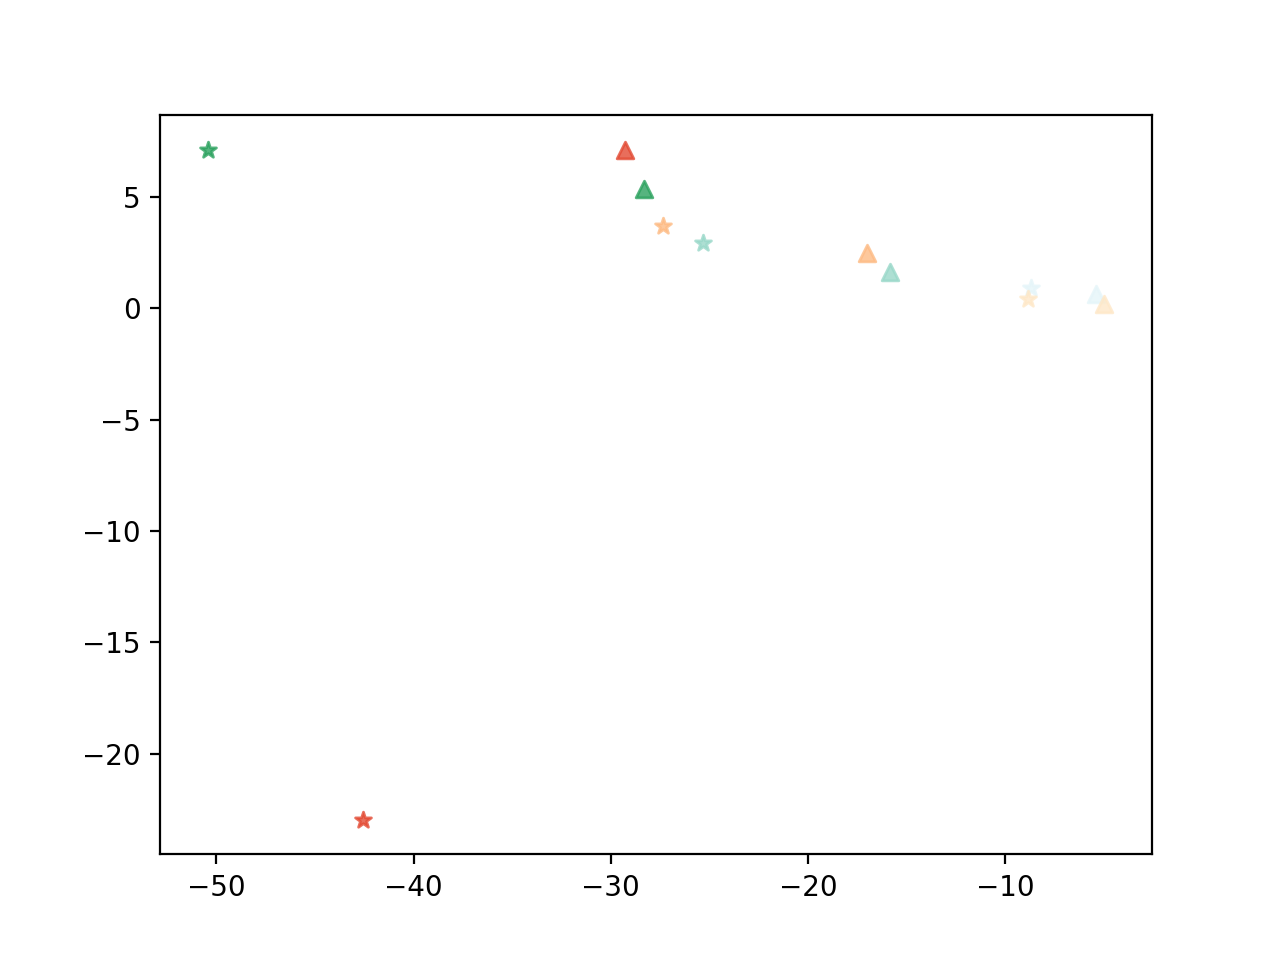
\includegraphics[width=\linewidth]{ms_linear}
        \caption{Linear Kernel}
    \end{subfigure}
    \begin{subfigure}[h]{0.3\textwidth}
        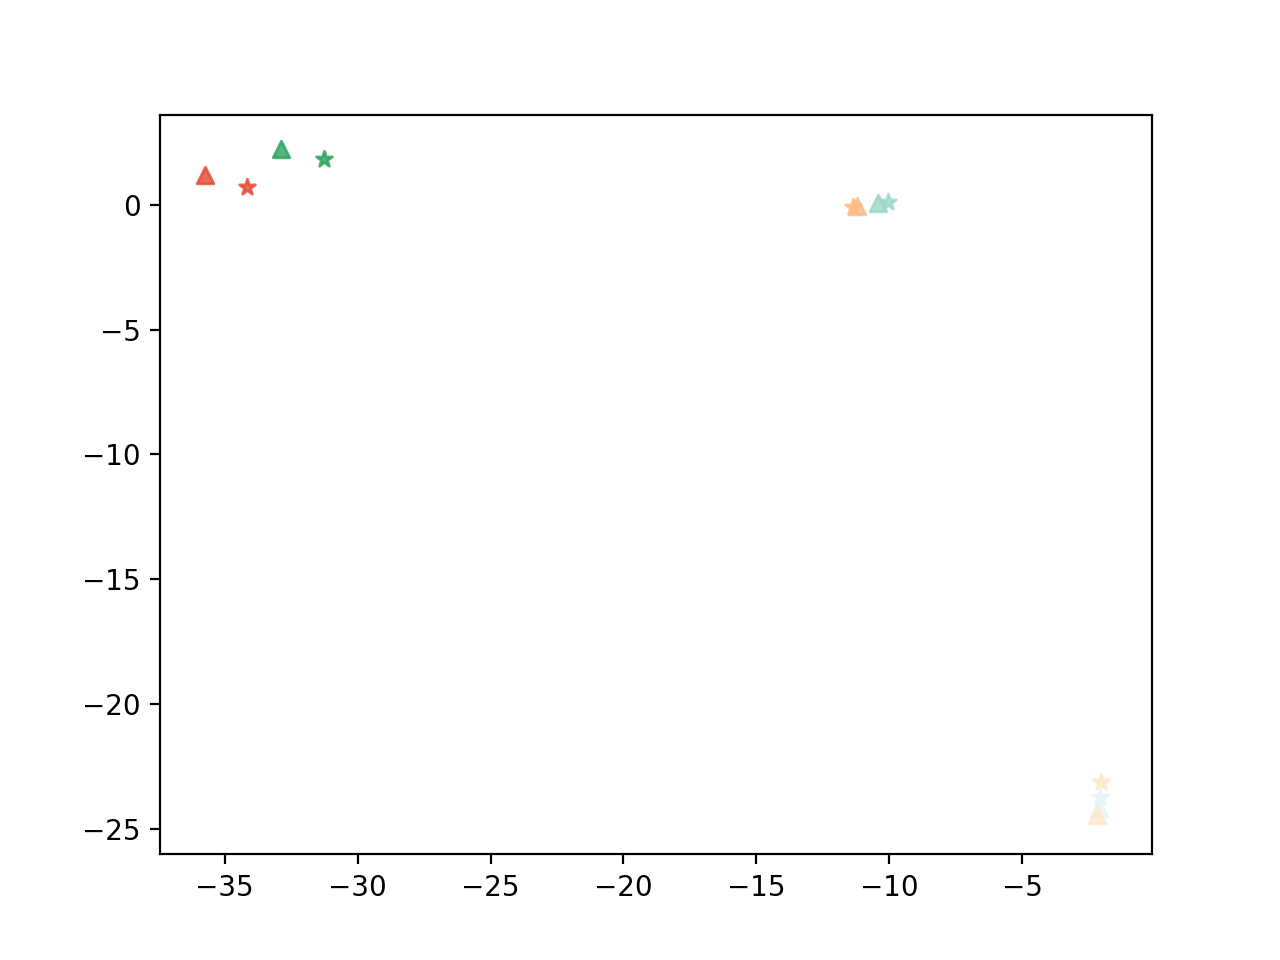
\includegraphics[width=\linewidth]{ms_smurf}
        \caption{SMURPH Kernel}
    \end{subfigure}%
    \begin{subfigure}[h]{0.3\textwidth}
        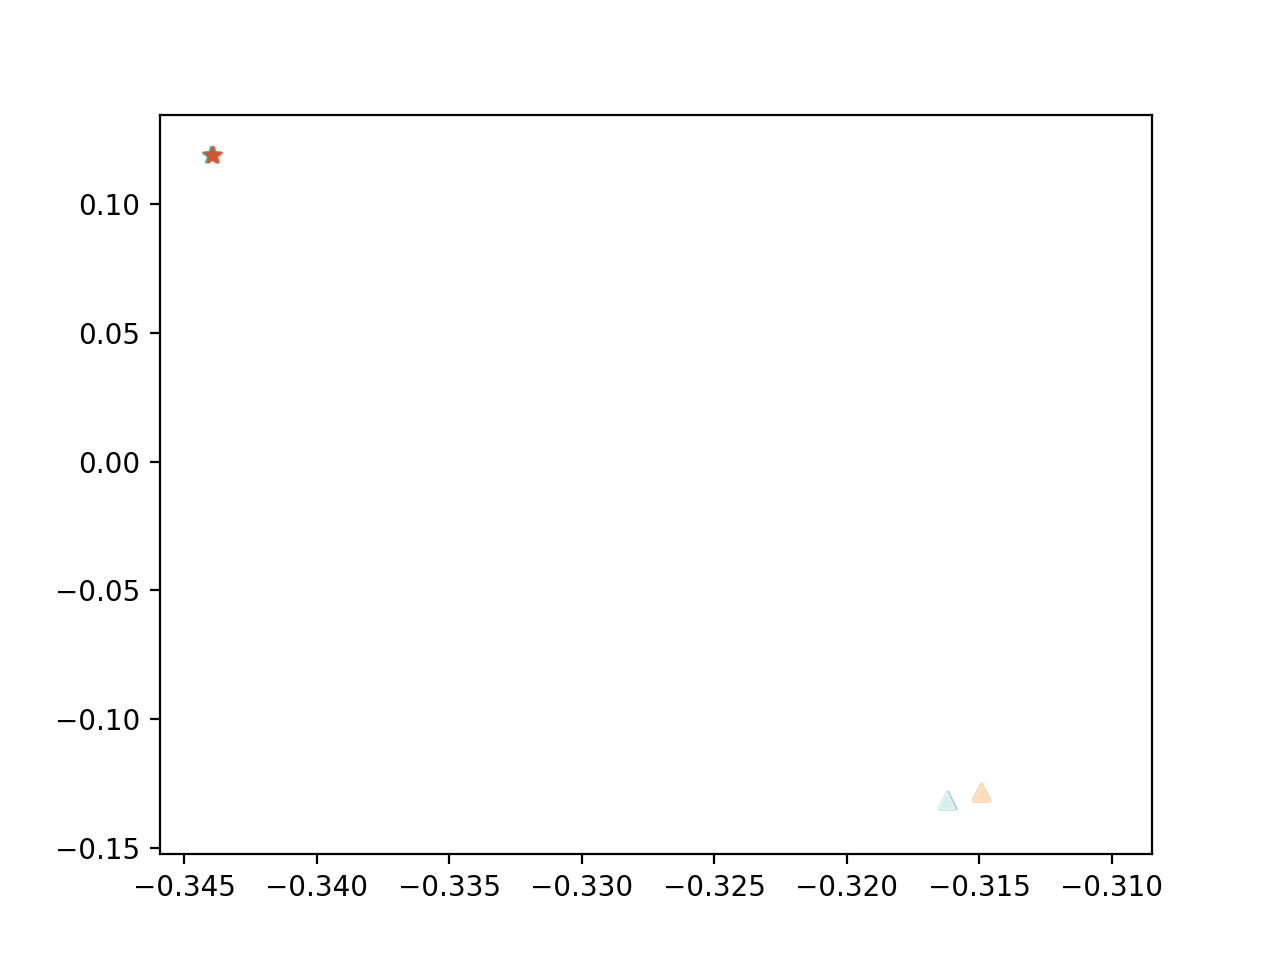
\includegraphics[width=\linewidth]{ms_hod}
        \caption{HOD Kernel}
    \end{subfigure}%
    \begin{subfigure}[h]{0.08\textwidth}
        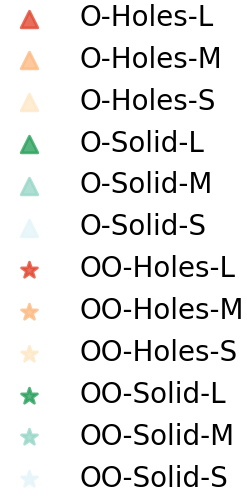
\includegraphics[width=\linewidth]{ms_legend}
    \end{subfigure}%
    \caption{Kernel PCA results for Synthetic Multiscale Dataset}
\end{figure}

\begin{figure}[H]
    \centering
    \begin{subfigure}[h]{0.4\textwidth}
        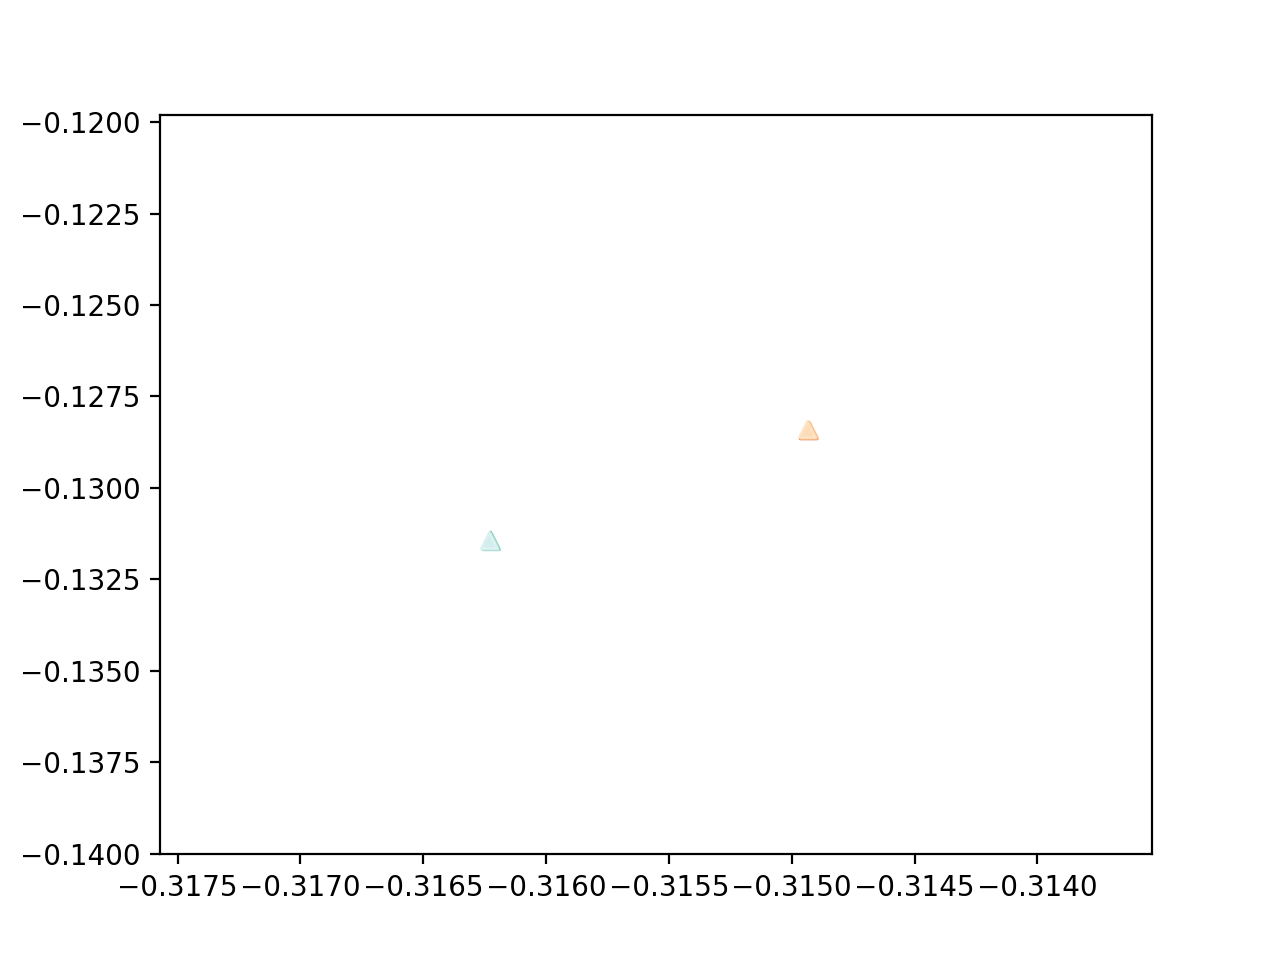
\includegraphics[width=\linewidth]{ms_hod_1}
        \caption{Bottom-right area}
    \end{subfigure}
    \begin{subfigure}[h]{0.4\textwidth}
        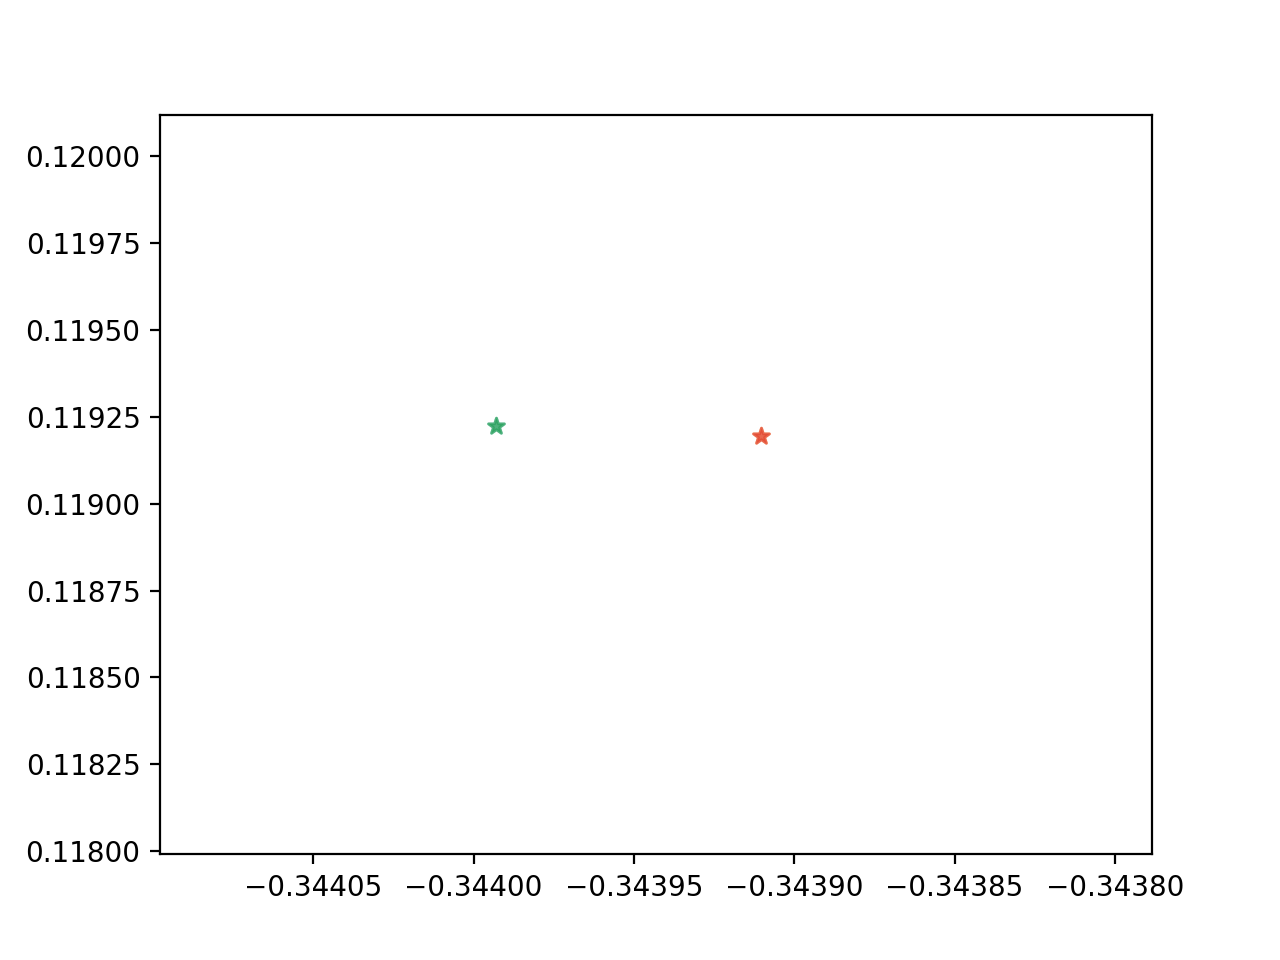
\includegraphics[width=\linewidth]{ms_hod_2}
        \caption{Top-left area}
    \end{subfigure}%
    \caption{HOD result zoom in}
\end{figure}

\section{Discussion}

\bibliographystyle{unsrt}
\bibliography{cites}
\end{document}
